%Use one of the two documentclass lines depending on aspect ratio needed
% for 4x3 aspect ratio slides
%\documentclass{beamer}
%for 16x9 (modern wide screen) aspect ratio slides
\documentclass[aspectratio=169]{beamer}

\setbeamercolor{block title}{fg=red,bg=white}
\setbeamercolor{block body}{fg=black,bg=red!10!white}

\makeatletter
\def\input@path{{templates/oxford-maths-slides/}}
\makeatother

\usepackage{mathtools}
\mathtoolsset{showonlyrefs}

% Oxford Maths theming
\usetheme{oxfordmaths}

\usepackage[backposition=title]{beamerappendixnote}
\usepackage{tikz}
\usetikzlibrary{calc,angles,quotes}
\usepackage{pgfplots}
\pgfplotsset{compat=1.18} % or your installed version
% Recommended preamble:
\usetikzlibrary{arrows.meta}
\usetikzlibrary{backgrounds}
\usepgfplotslibrary{patchplots}
\usepgfplotslibrary{fillbetween}
\pgfplotsset{%
    layers/standard/.define layer set={%
        background,axis background,axis grid,axis ticks,axis lines,axis tick labels,pre main,main,axis descriptions,axis foreground%
    }{
        grid style={/pgfplots/on layer=axis grid},%
        tick style={/pgfplots/on layer=axis ticks},%
        axis line style={/pgfplots/on layer=axis lines},%
        label style={/pgfplots/on layer=axis descriptions},%
        legend style={/pgfplots/on layer=axis descriptions},%
        title style={/pgfplots/on layer=axis descriptions},%
        colorbar style={/pgfplots/on layer=axis descriptions},%
        ticklabel style={/pgfplots/on layer=axis tick labels},%
        axis background@ style={/pgfplots/on layer=axis background},%
        3d box foreground style={/pgfplots/on layer=axis foreground},%
    },
}

\usepackage{appendixnumberbeamer}

\usepackage[
  backend=biber,
  style=authoryear,
  maxcitenames=1,
  url=false,
  doi=false,
  isbn=false,
  eprint=false
]{biblatex}

\addbibresource{references.bib}

\usepackage[abbreviations,automake]{glossaries-extra}

\newglossary[slg]{symbolslist}{syi}{syg}{List of Symbols}
\makeglossaries
\setabbreviationstyle{long-short}


\glsnoexpandfields

\newcommand*{\glsdefaultarg}{}
\newcommand*{\glsarg}{\glsdefaultarg}

\newglossaryentry{x}{
    category=arg,% requires an argument
    name=\ensuremath{\mathbold{x}_k},
    text=\mathbold{x}_{\glsarg},
    description={$k$th point in a sequence of iterations},
    type=symbolslist %in own list
}
\newglossaryentry{tily}{
    category=arg,% requires an argument
    name=\ensuremath{\tilde{y}^{(k)}},
    text=\tilde{y}^{(\glsarg)},
    description={Minimum norm point on affine subspace spanned by previous $\gls{x}[i]$},
    type=symbolslist %in own list
}
\newglossaryentry{y}{
    category=arg,% requires an argument
    name=\ensuremath{\mathbold{y}_k},
    text=\mathbold{y}_{\glsarg},
    description={Minimum norm vector in $\gls{aff}[\gls{R}]$},
    type=symbolslist %in own list
}
\newglossaryentry{aff}{
    %category=arg,% requires an argument
    name=\ensuremath{\operatorname{aff}(\cdot)},
    text=\operatorname{aff},
    description={Affine Hull},
    type=symbolslist %in own list
}
\newglossaryentry{su}{
    %category=arg,% requires an argument
    name=\ensuremath{\operatorname{su}(\cdot)},
    text=\operatorname{su},
    description={Sum of the argument's elements},
    type=symbolslist %in own list
}
\newglossaryentry{peninv}{
    category=arg,% requires an argument
    name=\ensuremath{(\cdot)^+},
    text=\glsarg^+,
    description={Moore-Penrose inverse, i.e. $\gls{peninv}[\gls{A}] = (\gls{A}^T\gls{A})^{-1}\gls{A}^T$},
    type=symbolslist %in own list
}
\newglossaryentry{F}{
    %category=arg,% requires an argument
    name=\ensuremath{\mathbold{F}},
    text=\mathbold{F},
    description={Generic fixed-point map. May or may not be linear.},
    type=symbolslist %in own list
}
\newglossaryentry{resF}{
    %category=arg,% requires an argument
    name=\ensuremath{\mathbold{G}},
    text=\mathbold{G},
    description={Generic residual map. May or may not be linear.},
    type=symbolslist %in own list
}
\newglossaryentry{Reals}{
    category=arg,% requires an argument
    name=\ensuremath{\mathbb{R}^{n}},
    text=\mathbb{R}^{\glsarg},
    description={$n$ dimensional Euclidean space},
    type=symbolslist %in own list
}
\newglossaryentry{Naturals}{
    %category=arg,% requires an argument
    name=\ensuremath{\mathbb{N}},
    text=\mathbb{N},
    description={Natural numbers},
    type=symbolslist %in own list
}
%\newcommand{\alphatwoargs}[1]{%
%  \StrBefore{#1}{,}[\firstarg]%
%  \StrBehind{#1}{,}[\secondarg]%
%  \alpha_{\firstarg\,\secondarg}%
%}
\newglossaryentry{alpha}{
    %category=arg,% requires an argument
    name=\ensuremath{\alpha},
    text=\alpha,
    description={Generic scalar},
    type=symbolslist %in own list
}
\newglossaryentry{r}{
    category=arg,% requires an argument
    name=\ensuremath{\mathbold{r}_{k}},
    text=\mathbold{r}_{\glsarg},
    description={$k$th residual in a sequence of iterations, i.e. $\gls{F}(\gls{x}[k]) - \gls{x}[k]$},
    type=symbolslist %in own list
}
\newglossaryentry{conv}{
    category=arg,% requires an argument
    name=\ensuremath{\varrho_k},
    text=\varrho_{\glsarg},
    description={$k$th root of convergence ratio, $\frac{\|\gls{r}[k]\|}{\|\gls{r}[0]\|}$},
    type=symbolslist %in own list
}
\newglossaryentry{rho}{
    category=arg,% requires an argument
    name=\ensuremath{\mathbold{\rho}_{k}},
    text=\mathbold{\rho}_{\glsarg},
    description={$k$th projection of the origin onto the affine subspace $\gls{R}[k]$},
    type=symbolslist %in own list
}
\newglossaryentry{Rmat}{
    category=arg,% requires an argument
    name=\ensuremath{\mathbold{R}_{k}},
    text=\mathbold{R}_{\glsarg},
    description={$k$th residual matrix containing the past $k$ iterates $\ges{r}[i]$, starting with the 0th!},
    type=symbolslist %in own list
}
\newglossaryentry{R}{
    category=arg,% requires an argument
    name=\ensuremath{\mathcal{R}_{k}},
    text=\mathcal{R}_{\glsarg},
    description={set of $k$ past residuals $\gls{r}_i$},
    type=symbolslist %in own list
}
\newglossaryentry{xstar}{
    %category=arg,% requires an argument
	name=\ensuremath{\mathbold{x}_{*}},
    text=\mathbold{x}_*,
    description={Generic fixed point},
    type=symbolslist %in own list
}
\newglossaryentry{A}{
    %category=arg,% requires an argument
    name=\ensuremath{\mathbold{A}},
    text=\mathbold{A},
    description={Generic linear map (matrix)},
    type=symbolslist %in own list
}
\newglossaryentry{V}{
    %category=arg,
    name={\ensuremath{\mathbold{V}}},
    text={\mathbold{V}},
    description={Matrix of eigenvectors}, %not sure about the order here yet!
    type=symbolslist
}
\newglossaryentry{Eig}{
    %category=arg,
    name={\ensuremath{\mathbold{\Lambda}}},
    text={\mathbold{\Lambda}},
    description={Diagonal matrix of eigenvalues}, %not sure about the order here yet!
    type=symbolslist
}
\newglossaryentry{EigSet}{
    %category=arg,
    name={\ensuremath{\Lambda}},
    text={\Lambda},
    description={Set of eigenvalues}, %not sure about the order here yet!
    type=symbolslist
}
\newglossaryentry{diag}{
    %category=arg,
    name={\ensuremath{\operatorname{diag}(\cdot)}},
    text={\operatorname{diag}},
    description={Diagonal matrix formed by putting the arguments on the diagonal}, %not sure about the order here yet!
    type=symbolslist
}

\newglossaryentry{I}{
    %category=arg,% requires an argument
    name=\ensuremath{\mathbold{I}},
    text=\mathbold{I},
    description={Identity matrix},
    type=symbolslist %in own list
}

\newglossaryentry{a}{
    %category=arg,% requires an argument
    name=\ensuremath{a},
    text=a,
    description={Generic vector},
    type=symbolslist %in own list
}
\newglossaryentry{b}{
    %category=arg,% requires an argument
    name=\ensuremath{\mathbold{b}},
    text=\mathbold{b},
    description={Generic vector},
    type=symbolslist %in own list
}

\newglossaryentry{S}{
    %category=arg,% requires an argument
    name=\ensuremath{\mathcal{S}},
    text=\mathcal{S},
    description={Generic set},
    type=symbolslist %in own list
}
% Generic macro to support 1 to 3 arguments for a symbol
\newglossaryentry{K}{
    category=arg,
    name={\ensuremath{\mathcal{K}_{n}}},
    text={\mathcal{K}_{\glsarg}},
    description={Order-$n$ Krylov subspace, optional arguments specify matrix and vector},
    type=symbolslist
}
\newglossaryentry{Kmat}{
    category=arg,
    name={\ensuremath{\mathbold{K}_{n}}},
    text={\mathbold{K}_{\glsarg}},
    description={Order-$n$ Krylov subspace, optional arguments specify matrix and vector},
    type=symbolslist
}
\newglossaryentry{G}{
    category=arg,
    name={\ensuremath{\mathbold{G}_{n}}},
    text={\mathbold{G}_{\glsarg}},
    description={Order-$n$ Krylov subspace Gramiam Matrix, optional arguments specify matrix and vector},
    type=symbolslist
}
\newglossaryentry{Gdet}{
    category=arg,
    name={\ensuremath{\gamma_{n}}},
    text={\gamma_{\glsarg}},
    description={Order-$n$ Krylov subspace Gramiam Matrix determinant, optional arguments specify matrix and vector},
    type=symbolslist
}
\newglossaryentry{Paff}{
    category=arg,
    name={\ensuremath{\mathcal{P}_{n}^{\mathrm{aff}}}},
    text={\mathcal{P}_{\glsarg}^{\mathrm{aff}}},
    description={Set of polynomials of order $n-1$ whose coefficients sum to 1}, %not sure about the order here yet!
    type=symbolslist
}
\newglossaryentry{p}{
    category=arg,
    name={\ensuremath{p_{n}}},
    text={p_{\glsarg}},
    description={Generic polynomials of order $n-1$}, %not sure about the order here yet!
    type=symbolslist
}
\newglossaryentry{q}{
    category=arg,
    name={\ensuremath{q_{n}}},
    text={q_{\glsarg}},
    description={A generic polynomials of order $n-1$}, %not sure about the order here yet!
    type=symbolslist
}
\newglossaryentry{eig}{
    category=arg,
    name={\ensuremath{\lambda_{i}}},
    text={\lambda_{\glsarg}},
    description={A diagonal entry in a matrix $\gls{Eig}$}, %not sure about the order here yet!
    type=symbolslist
}
\newglossaryentry{cond}{
    %category=arg,
    name={\ensuremath{\kappa(\cdot)}},
    text={\kappa},
    description={2-norm condition number}, %not sure about the order here yet!
    type=symbolslist
}
\newglossaryentry{T}{
    category=arg,
    name={\ensuremath{T_{k}(z)}},
    text={T_{\glsarg}},
    description={standard $k$th Chebyshev polynomial of the first kind.}, %not sure about the order here yet!
    type=symbolslist
}
\newglossaryentry{emin}{
    %category=arg,
    name={\ensuremath{\lambda_{\text{min}}}},
    text={\lambda_{\text{min}}},
    description={Minimum eigenvalue}, %not sure about the order here yet!
    type=symbolslist
}
\newglossaryentry{emax}{
    %category=arg,
    name={\ensuremath{\lambda_{\text{max}}}},
    text={\lambda_{\text{max}}},
    description={Maximum eigenvalue}, %not sure about the order here yet!
    type=symbolslist
}
\newglossaryentry{e}{
    %category=arg,
    name={\ensuremath{\mathbold{e}}},
    text={\mathbold{e}},
    description={Vector of 1s}, %not sure about the order here yet!
    type=symbolslist
}
\newglossaryentry{eps}{
    category=arg,% requires an argument
    name=\ensuremath{\mathbold{\epsilon}_k},
    text=\mathbold{\epsilon}_{\glsarg},
    description={Error vector},
    type=symbolslist %in own list
}
\newglossaryentry{m}{
    %category=arg,
    name={\ensuremath{\mu}},
    text={\mu},
    description={History parameters of \glsxtrlong{raa} and \glsxtrlong{waa}}, %not sure about the order here yet!
    type=symbolslist
}
\newglossaryentry{vecalpha}{
    %category=arg,
    name={\ensuremath{\mathbold{\alpha}_k}},
    text={\mathbold{\alpha}},
    description={$k$th vector of coefficients}, %not sure about the order here yet!
    type=symbolslist
}

\newabbreviation{gmres}{GMRES}{generalised minimal residual method}
\newabbreviation{aa}{AA}{Anderson acceleration}
\newabbreviation{pi}{PI}{Picard iteration}
\newabbreviation{sdp}{SDP}{semidefinite programming problem}
\newabbreviation{esm}{ESM}{Earth system model}
\newabbreviation{raa}{rAA}{restarted \gls{aa}}
\newabbreviation{waa}{wAA}{windowed \gls{aa}}
\newabbreviation{cg}{CG}{conjugate gradient}


\preto\glsentryfmt{%
  \glsifcategory{\glslabel}{arg}% if category set to "arg"
  {%
    \ifdefempty\glsinsert
    {\let\glsarg\glsdefaultarg}%
    {%
      \let\glsarg\glsinsert
      \let\glsinsert\empty
    }%
  }%
  {}%
}

\usepackage{fixmath}

% Set author etc info
\title[AA Convergence] %short version of title for slide footer
{Rates of Convergence of Anderson Acceleration for 
 Fixed Point Problems \emph{(in preparation)}} %full title for titlepage
\author{\emph{Tobias Bretschneider} and Coralia Cartis}
\institute{Mathematical Institute\\University of Oxford\\United Kingdom}
\date[Wed 4 June 2026]  %short date for slide footer
{SIAM Conference on Optimization (OP26), June 2026 \\
Wednesday, June 3 \\ MS121 \\
Inexact and Accelerated Methods for Nonlinear Problems} %main date for title page,
                        %can overload it to show say 'Conference X, Date Y'


%% Now for the actual slides %%
\begin{document}

\begin{frame}[plain]
  \titlepage
\end{frame}

\begin{frame}{Fixed-point problems}
    \begin{itemize}
        \item Given a function $\gls{F} :\gls{Reals}[n] \to \gls{Reals}[n]$ we want to
            find an approximate fixed-point $\gls{x}[*]\in\gls{Reals}[n]$ s.t.
            $\gls{F}(\gls{x}[*]) \approx \gls{x}[*]$.
        \item \gls{pi} would produce a sequence of iterates
            $(\gls{x}_i^\text{\gls{pi}})_{i \in \gls{Naturals}}$ by starting with
            initial guess $\gls{x}[0]$ and repeatedly applying $\gls{F}$, 
            \begin{equation}
                \gls{x}_{i+1}^\text{\gls{pi}} = \gls{F}(\gls{x}_i^\text{\gls{pi}}).
            \end{equation}
        \item \gls{pi} only works for contractive $\gls{F}$, and can have slow
            convergence. 
        \item {\color{red}\emph{Idea: Can we utilise the history to have an idea of
            where we are going?}}
    \end{itemize}
\end{frame}

\begin{frame}{\only<2>{{\color{red} Infinite History }}%
            \only<3>{{\color{red} Restarted }}%
            \only<4>{{\color{red} Windowed }}%
            \only<5>{{\color{red} Alternating \gls{pi} }}%
            \glsfirst{aa}}
    
        % \only<1>{\item Under ``linearisation'' combining past iterates such that their
        %     ``combined'' residuals are small should be good.}
        \only<1-4>{\only<1>{\gls{aa} each time takes a linear combination of multiple previous
            iterates. It p}\only<2->{P}roduces a sequence, $(\gls{x}[i])_{i \in \gls{Naturals}}$
            with,
            \begin{equation}\label{eqn:simpaaform}
                \gls{x}[i+1] = \only<1>{\sum_{j}}
                            \only<2>{\sum_{{\color{red} j=0}}^{{\color{red} i}}}
                            \only<3>{\sum_{{\color{red} j=i-(i \bmod m)}}^{{\color{red} i}}}
                            \only<4>{\sum_{{\color{red} j=i-m_k+1}}^{{\color{red} i}}}
                \gls{alpha}_j \gls{F}(\gls{x}[j]),
            \end{equation}
            for coefficients $\gls{alpha}_j$, (computed at each step) solving,
            \begin{equation}
                \gls{vecalpha} =  \operatorname*{arg\,min}_{\gls{vecalpha} \text{ st.}
                \sum_j
                \gls{alpha}_j = 1} \left\|%
                    \only<1>{\sum_j}
                    \only<2>{\sum_{{\color{red} j=0}}^{{\color{red} i}}}
                    \only<3>{\sum_{{\color{red} j=i - (i \bmod m)}}^{{\color{red} i}}}
                    \only<4>{\sum_{{\color{red} j=i-m_k+1}}^{{\color{red} i}}}
                \gls{alpha}_j \gls{r}[j]\right\|.
            \end{equation}
            \only<4>{\color{red}($m_k = \min \{m,k\}$)}}
        \only<1>{Where we introduce the residual at each step, $\gls{r}[i] := \gls{F}(\gls{x}_i) -
            \gls{x}_i$; a measure of deviation from the fixed-point.}
        \only<2>{{\color{red} Uses all the past residuals.}}
        \only<3>{{\color{red} Clears the history every $m$ steps.}}
        \only<4>{{\color{red} Keeps a maximum history of size $m$, always deleting oldest if it gets too big.}}
        %\only<5>{\item {\color{red} Takes $k$ \gls{pi} steps inbetween each \gls{aa}
        %    update (can also be combined with other variants).}}
\end{frame}

\begin{frame}{Convergence of \gls{aa}}
    \begin{itemize}
        \item Proven that \gls{aa} converges when the fixed-point map is contractive
            \parencite{Toth2015}; \only<1>{\color{red} no improvement over \gls{pi}.} \pause
        \item Shown that \gls{aa} is no worse than \gls{pi} \parencite{Evans2020};
            \only<2>{\color{red} no results showning in which cases it is strictly
            better.} \pause 
        %\item \cite{d_Aspremont2021} results similar to Krylov analysis of GMRES.
        \item  \parencite{Garner2023} shows strict improvement bounds  for windowed \gls{aa};  \pause
        \item  \parencite{De_Sterck2022}:  explicit convergence rates  for restarted \gls{aa} on further normal
            linear systems. \pause
        \item {\color{red} We still don't have a full appreciation of when, and to what
            extent \gls{aa} (any variant) improves upon \gls{pi} (even when applied to
            \textbf{linear maps}).}
    \end{itemize}
\end{frame}

% \begin{frame}{Simplification in the Linear Case}
%     \begin{itemize}
%         \item Consider an affine fixed-point map $\gls{F}(\gls{x}) = \gls{A}\gls{x}
%             + \gls{b}$, with fixed-point $\gls{xstar}$ (satisfying $
%             \gls{F}(\gls{xstar})=\gls{xstar}$). 
%         \item We can in fact WLOG let $\gls{b} = 0$.
%             \begin{itemize}
%                 \item Define the error as $\gls{eps}[k] := \gls{x}[k]-\gls{xstar}$.
%                 \item Since $\gls{xstar} = \gls{A}\gls{xstar}+ \gls{b}$, we have that,
%                     \begin{equation}
%                         \gls{eps}[k+1] = \gls{A}\gls{eps}[k].
%                     \end{equation}
%             \end{itemize}
%     \end{itemize}
%     \appxnote{Shift details}{
%         Note that subtracting $\gls{xstar}$ off the Picard iteration gives,
%         \begin{equation}
%             \gls{eps}[k+1] = \gls{F}(\gls{x}[k]) -
%             \gls{xstar}.
%         \end{equation}
%         Then using the defining property of $\gls{xstar} = \gls{A}\gls{xstar} -
%         \gls{b}$, and expanding $\gls{F}$,
%         \begin{equation}
%             \gls{eps}[k+1] = \gls{A}\gls{x}[k]+ \gls{b} -
%             A\gls{xstar}-\gls{b}.
%         \end{equation}
%         Which gives, as desired,
%         \begin{equation}
%             \gls{eps}[k+1] = \gls{A}(\gls{x}[k]-\gls{xstar}) =
%             \gls{A}\gls{eps}[k].
%         \end{equation}
%     }
% \end{frame}

\begin{frame}{Simplification for Linear Case}
    For a linear map\footnote{this includes affine maps (after translation behaviour is
    identical).}, $\gls{F}(\gls{x}) = \gls{A}\gls{x}$, \gls{aa} is equivalent to a
    simple update on residuals:
    \begin{block}{}
    \begin{enumerate}
        \item Calculate $\gls{rho}[i+1]$ given by,
        \begin{equation}
            \gls{rho}[i+1] = \operatorname*{arg\,min}_{\mathbold{v} \in \gls{aff}(\gls{R}[i+1])}
            \|\mathbold{v}\|, \quad \text{where $\gls{R}[i+1] = \{\gls{r}[0], \dots,
            \gls{r}[i]\}$,}
        \end{equation}
        \item Calculate $\gls{r}[i+1]$ from,
            \begin{equation}
            \gls{r}[i+1] = \gls{A} \gls{rho}[i+1].
            \end{equation}
    \end{enumerate}
    \end{block}
    Initial residual is $\gls{r}[0] = (\gls{A}-\gls{I})\gls{x}[0]$.

    {\footnotesize Simplifications come as $\gls{A}-\gls{I}$ and $\gls{A}$ commute. Computing the
    residual commutes with applying the map. More details in \parencite{Garner2023}}
    % \appxnote{Residual map equivalency details}{
    %     We have
    %     \begin{multline}
    %         \gls{r}[i+1] = (\gls{A}-\gls{I}) \gls{x}[i+1] =
    %         (\gls{A}-\gls{I})\sum_j \gls{alpha}_j \gls{A} \gls{x}[j] = \\ =
    %         \gls{A}\sum_{j} \gls{alpha}_j (\gls{A}-\gls{I})(\gls{x}[j]) =
    %         \gls{A} \sum_{j} \gls{alpha}_j \gls{r}[j] = \gls{A}
    %         \gls{rho}[i+1],
    %     \end{multline}
    %     where we have defined $\gls{rho}[j+1]$ as the point with minimum
    %     norm on the affine hull of previous residuals. In the infinite
    %     history case, if we let $\gls{R}[i+1]$ denote the set of past $i+1$
    %     residuals this can be written as
    %     \begin{equation}
    %         \gls{rho}[i+1] = \operatorname*{arg\,min}_{\mathbold{v} \in
    %         \gls{aff}(\gls{R}[i+1])} \|\mathbold{v}\|,
    %     \end{equation}
    %     where $\gls{aff}(\gls{R}[i+1])$ is the affine hull of past residuals.
    %     }
\end{frame}


\begin{frame}{Solving the minimisation problem}
    We have 
    \begin{equation}\label{eqn:rhonorm}
        \|\gls{rho}[k]\|^2 = \frac{1}{\gls{e}^T(\gls{Rmat}[k]^T\gls{Rmat}[k])^{-1}\gls{e}},
    \end{equation}
    where $\gls{e}$ is an appropriately sized vector of ones (so we have the sum of the
    entries of $(\gls{Rmat}[k]^T\gls{Rmat}[k])^{-1}$), and
    \begin{equation}\gls{Rmat}[k] = \begin{bmatrix}
        \gls{r}[0] & \gls{r}[1] & \cdots & \gls{r}[k-1]
    \end{bmatrix},
    \end{equation}
    the matrix of past $k$ residuals.\hfill  {\footnotesize Details in \parencite{Ni2009}}

    % \appxnote{Minimum norm proof}{
    %     \begin{proof}
    %         The vector of coefficients, $\gls{vecalpha}$, in expansion of $\gls{rho}[k]$
    %         on the previous $k$ residuals is derived using Lagrange multipliers, details
    %         of which can be found for example in \cite{Ni2009}. It is given by
    %         \begin{equation}\label{eqn:vecalpha}
    %             \gls{vecalpha} =
    %             \frac{(\gls{Rmat}[k]^T\gls{Rmat}[k])^{-1}\gls{e}}{\gls{e}^T(\gls{Rmat}[k]^T\gls{Rmat}[k])^{-1}\gls{e}}.
    %         \end{equation}
    %         Since $\gls{rho}[k] = \gls{Rmat}[k]\gls{vecalpha}$,
    %         we have that
    %         \begin{multline}
    %             \|\gls{rho}[k]\|^2 =
    %             \gls{vecalpha}^T\gls{Rmat}[k]^T\gls{Rmat}[k]\gls{vecalpha} =
    %             \frac{\gls{e}^T(\gls{Rmat}[k]^T\gls{Rmat}[k])^{-1}\gls{Rmat}[k]^T\gls{Rmat}[k](\gls{Rmat}[k]^T\gls{Rmat}[k])^{-1}\gls{e}}{\left(\gls{e}^T(\gls{Rmat}[k]^T\gls{Rmat}[k])^{-1}\gls{e}\right)^2}
    %             = \\ =
    %             \frac{\gls{e}^T(\gls{Rmat}[k]^T\gls{Rmat}[k])^{-1}\gls{e}}{\left(\gls{e}^T(\gls{Rmat}[k]^T\gls{Rmat}[k])^{-1}\gls{e}\right)^2}.
    %         \end{multline}
    %     \end{proof}
    % }
\end{frame}

\begin{frame}{Affine hull equivalences}

Four sets of vectors:
\begin{itemize}
    \item residual vectors, $\gls{R}[n] = \{\gls{r}[0],\gls{r}[1],\dots, \gls{r}[n-1]\};$
    \item Krylov vectors, $\gls{K}[n] %= \gls{K}[n](\gls{A},\gls{r}[0]) 
    = \{ \gls{r}[0], \gls{A} \gls{r}[0], \ldots, \gls{A}^{n-1} \gls{r}[0] \}$; and,
    \item minimisation problem solutions, $\gls{M}[n] =
        \{\gls{rho}[1],\gls{rho}[2],\dots, \gls{rho}[n-1], \gls{rho}[n]\}.$
    \item minimisation problem solutions + current residual, $\gls{Mtilde}[n] =
        \{\gls{rho}[1],\gls{rho}[2],\dots, \gls{rho}[n-1], \gls{r}[n-1]\}.$
\end{itemize}
\parencite{Bretschneider2025} All their affine hulls are equivalent,
\begin{equation}
    \gls{aff}(\gls{K}[n]) = \gls{aff}(\gls{R}[n]) = \gls{aff}(\gls{Mtilde}[n]) = \gls{aff}(\gls{M}[n]),
\end{equation}
assuming stagnation, $\gls{r}[i] = \gls{r}[i+1]$ does not happen\footnote{The
    possibility of stagnation during \gls{aa} has been covered in detail in
    \parencite{Potra2011}.}.

% \appxnote[allowframebreaks]{Hull equivalency proofs}{
%     We use induction. For $n=1$,
%     \begin{equation}
%         \gls{K}[1] = \gls{R}[1] = \gls{M}[1] = \gls{Mtilde}[1] = \{\gls{r}[0]\}.
%     \end{equation}
%
%     Assume now that $ \gls{aff}(\gls{K}[n]) = \gls{aff}(\gls{R}[n]) =
%     \gls{aff}(\gls{Mtilde}[n]) = \gls{aff}(\gls{M}[n])$.
%
%     By definition $ \gls{rho}[n] \in \gls{aff}(\gls{R}[n])$. But also by the induction
%     hypothesis, $\gls{rho}[n] \in \gls{aff}(\gls{K}[n]).$ Applying $\gls{A}$ gives $
%     \gls{r}[n] = \gls{A}\gls{rho}[n] \in \gls{aff}(\gls{K}[n+1]), $ since $\gls{A}$ is
%     linear so affine coefficients will be preserved!
%
%     Therefore
%     \begin{equation}
%         \gls{aff}(\gls{R}[n+1]) \subseteq \gls{aff}(\gls{K}[n+1]).
%     \end{equation}
%
%     Further, by induction, $\gls{aff}(\gls{M}[n]) = \gls{aff}(\gls{R}[n])$, so indeed,
%     $\gls{aff}(\gls{Mtilde}[n+1]) = \gls{aff}(\gls{R}[n+1])$. Moreover as
%     $\gls{rho}[n+1] \in \gls{R}[n+1]$, we have that,
%     \begin{equation}
%         \gls{M}[n+1] \subseteq \gls{Mtilde}[n+1] = \gls{R}[n+1] \subseteq \gls{K}[n+1].
%     \end{equation}
%
%     Now we have, $\gls{rho}[n+1] \in \gls{aff}(\gls{M}[n+1]) \subseteq
%     \gls{aff}(\gls{R}[n+1])$, so,
%     \begin{equation}
%         \gls{rho}[n+1] = \beta_0 \mathbold{v} + \beta_1 \gls{r}[n],
%     \end{equation}
%     where $\mathbold{v} \in \gls{aff}(\gls{R}[n]) = \gls{aff}(\gls{M}[n])$ and $\beta_0
%     + \beta_1 = 1$. Moreover $\beta_1 \neq 0$ since we have explicitly discounted
%     stagnation. Rearranging gives,
%     \begin{equation}
%         \label{eqn:affequivrearrangedi}
%         \gls{r}[n] = \frac{1}{\beta_1} \gls{rho}[n+1] -
%         \frac{\beta_0}{\beta_1}\mathbold{v} \in \gls{aff}(\gls{M}[n+1]),
%     \end{equation}
%     since, $\frac{1}{\beta_1} - \frac{\beta_0}{\beta_1} = 1$.
%     Finally we have, $\gls{rho}[n] \in \gls{aff}(\gls{M}[n]) = \gls{aff}(\gls{K}[n])$,
%     so,
%     \begin{equation}
%         \gls{rho}[n] = \beta_0 \mathbold{v} + \beta_1 \gls{A}^{n-1} \gls{r}[0],
%     \end{equation}
%     where $\mathbold{v} \in \gls{aff}(\gls{K}[n -1])$ and $\gamma_0 + \gamma_1 = 1$.
%     Moreover $\gamma_1 \neq 0$ since we have explicitly discounted stagnation.
%     Multiplying by $\gls{A}$ and rearranging gives,
%     \begin{equation}
%         \label{eqn:affequivrearranged}
%         \gls{A}^n \gls{r}[0] = \frac{1}{\gamma_1} \gls{r}[n] -
%         \frac{\gamma_0}{\gamma_1}\gls{A}\mathbold{v},
%     \end{equation}
%     so, because $\gls{A}\mathbold{v} \in \gls{aff}(\gls{K}[n]) = \gls{aff}(\gls{R}[n])$
%     and $\frac{1}{\gamma_1} - \frac{\gamma_0}{\gamma_1} = 1$, shows that $\gls{A}^n
%     \gls{r}[0] \in \gls{aff}(\gls{R}[n+1])$. Thus finally we have the desired result.
%     }
\end{frame}

\begin{frame}{Using equivalence on the minimisation problem}

    Now if we consider the matrices, $\gls{Rmat}[k],\gls{Kmat}[k],\gls{Mmat}[k]$ ,
    corresponding to the sets, $\gls{R}[k],\gls{K}[k],\gls{M}[k]$, we have,

        \begin{equation}\label{eqn:rhonormi}
        \|\gls{rho}[k]\|^2 =
            \frac{1}{\gls{e}^T(\gls{Rmat}[k]^T\gls{Rmat}[k])^{-1}\gls{e}} =
            \frac{1}{\gls{e}^T(\gls{Kmat}[k]^T\gls{Kmat}[k])^{-1}\gls{e}} =
            \frac{1}{\gls{e}^T(\gls{Mmat}[k]^T\gls{Mmat}[k])^{-1}\gls{e}}.
    \end{equation}
    \pause
    \begin{block}{}
    We now follow with two analysis approaches based on different equivalences: 
        \begin{itemize}
            \item Approach I: using the equivalence to a Krylov method,
            \item Approach II: a more geometric approach.
        \end{itemize}
    \end{block}
\end{frame}

\begin{frame}{Approach I: Krylov/Polynomial}

    The affine equivalence lets us phrase the minimum norm problem as,
    \begin{equation}
        \gls{rho}[k] = \operatorname*{arg\,min}_{\mathbold{v} \in \gls{aff}(\gls{R}[k])}
        \|\mathbold{v}\| = \operatorname*{arg\,min}_{\mathbold{v} \in \gls{aff}(\gls{K}[k])}
        \|\mathbold{v}\| = \operatorname*{arg\,min}_{p \in \gls{Paff}[k]}
        \|p(\gls{A})\gls{r}[0]\|.
    \end{equation}

    Where,
    \begin{equation}
        \gls{Paff}[n] = \{\text{polynomials $p$ of degree $< n$ with $p(1)=1$}\}.
    \end{equation}

    {\footnotesize Very well known in the GMRES literature, carried over to \gls{aa} in
    \parencite{d_Aspremont2021}}

\end{frame}

\begin{frame}{Explicit evaluations}
    \only<1>{
    They are all very similar to typical GMRES computations. Symmetric and
    Skew-symmetric cases let us analytically write down bounds based on Tchebyshev
    polynomials. General case can be covered by an SDP optimisation program.}

    \only<2>{
    \begin{theorem}\label{thm:symcase}\cite{Bretschneider2025} For \gls{aa} applied to a symmetric matrix
        $\gls{A}$ with eigenvalues contained in the interval $[\gls{emin},\gls{emax}]$
        and 1 not in this interval we have
        \begin{equation}
            \frac{\|\gls{r}[k]\|}{\|\gls{r}[0]\|} \leq
            \frac{2\max\{|\gls{emin}|,|\gls{emax}|\}}{y^{k-1} + y^{-k+1}},
        \end{equation}
        where $y = |1+2w|+2\sqrt{w^2+w}$, with $w = \frac{1 -\gls{emax}}{\gls{emax}
        -\gls{emin}}$.
    \end{theorem}
    }

    \only<3>{
    \begin{theorem}\label{thm:polyskewsym}
        \parencite{Bretschneider2025} For \gls{aa} applied to a skew-symmetric $\gls{A}$ with $\|\gls{A}\|\leq
        \gls{emax}$ we have
        \begin{equation}
            \frac{\|\gls{r}[2m+1]\|}{\|\gls{r}[0]\|} \leq
            \frac{2\gls{emax}}{y^{2m}+y^{-2m}},
        \end{equation}
        \begin{equation}
            \frac{\|\gls{r}[2m]\|}{\|\gls{r}[0]\|} \leq
            \frac{2\gls{emax}}{y^{2m-1}-y^{-2m+1}},
        \end{equation}
        where
        \begin{equation}
            y = \frac{1}{\gls{emax}} + \sqrt{\frac{1}{\gls{emax}^2}+1}.
        \end{equation}
    \end{theorem}
    }
\end{frame}

\begin{frame}{Symmetric case visualisation}
    \begin{figure}
        \centering
        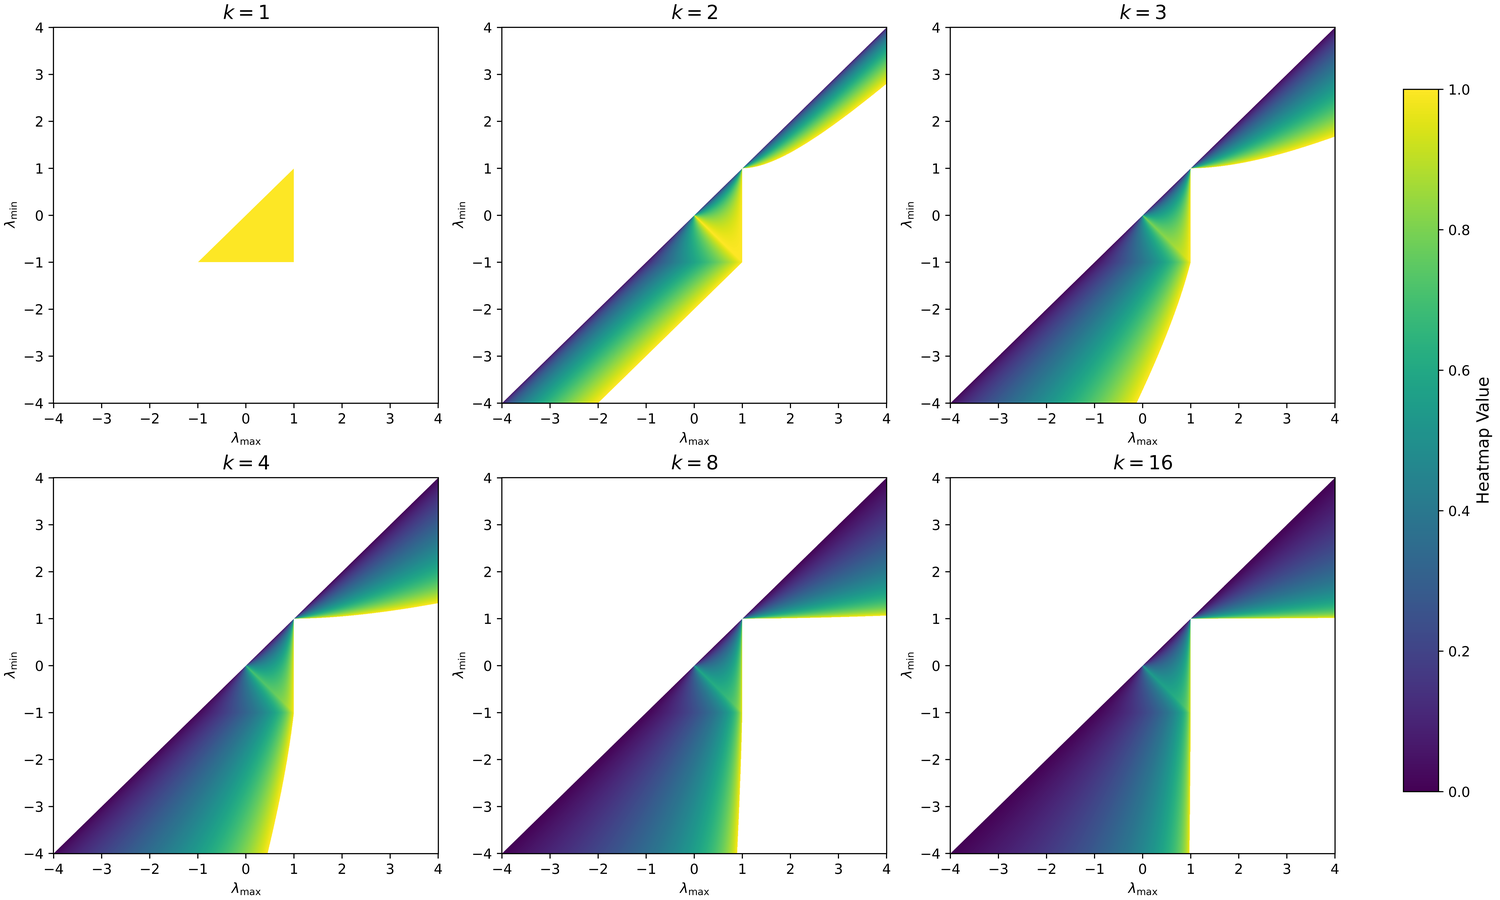
\includegraphics[width=0.8\linewidth]{images/pngs/symmetric_heatmap_grid_small.png}
        % \caption{Collection of heatmaps for different $k$ values. Plotted over of
        % $\gls{emax}$ and $\gls{emin}$. On the square $[ -1,1] \times [ -1,1]$ the ratio
        % $\gls{conv}_k/\gls{conv}_k^{\text{\gls{pi}}}$ is plotted and outside this square
        % just $\gls{conv}_k$ is plotted.}
        \label{fig:heatmapsym}
    \end{figure}
\end{frame}

\begin{frame}{Evaluation of Polynomial style bounds}
    \only<1,3>{
    \begin{itemize}
        \item This leads to very well-known GMRES style bounds.
        \item Can show certain types of maps always converge even if Picard does not.
        \item Can demonstrate improvement for certain classes of maps.
        \item Improves upon work in \parencite{Krzysik2025}, but approach noted in
            \parencite{d_Aspremont2021}.
    \end{itemize}
    }
    \only<2>{
        \begin{figure}
            \begin{center}
                % Recommended preamble:
% \usetikzlibrary{arrows.meta}
% \usetikzlibrary{backgrounds}
% \usepgfplotslibrary{patchplots}
% \usepgfplotslibrary{fillbetween}
% \pgfplotsset{%
%     layers/standard/.define layer set={%
%         background,axis background,axis grid,axis ticks,axis lines,axis tick labels,pre main,main,axis descriptions,axis foreground%
%     }{
%         grid style={/pgfplots/on layer=axis grid},%
%         tick style={/pgfplots/on layer=axis ticks},%
%         axis line style={/pgfplots/on layer=axis lines},%
%         label style={/pgfplots/on layer=axis descriptions},%
%         legend style={/pgfplots/on layer=axis descriptions},%
%         title style={/pgfplots/on layer=axis descriptions},%
%         colorbar style={/pgfplots/on layer=axis descriptions},%
%         ticklabel style={/pgfplots/on layer=axis tick labels},%
%         axis background@ style={/pgfplots/on layer=axis background},%
%         3d box foreground style={/pgfplots/on layer=axis foreground},%
%     },
% }

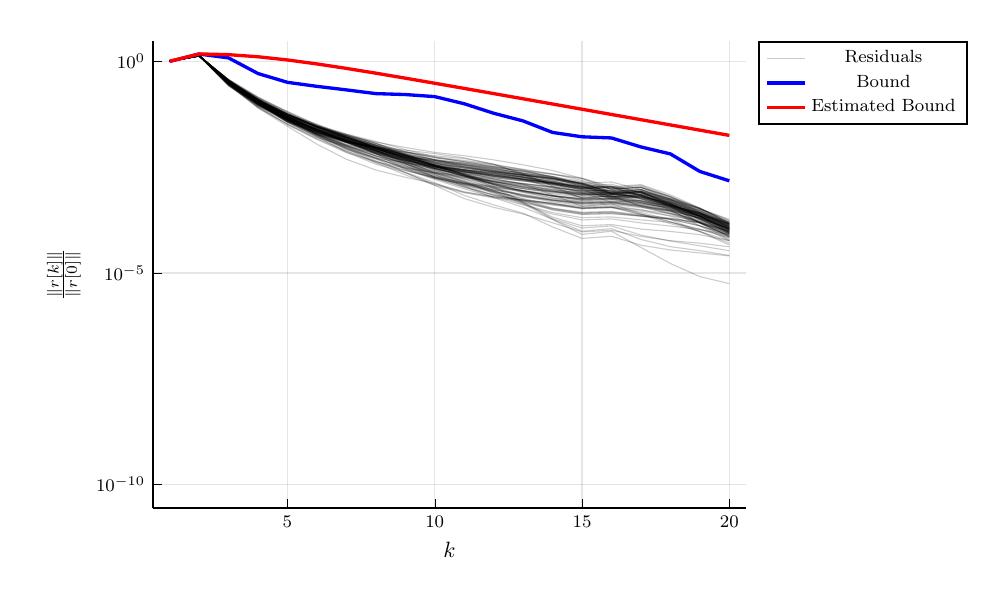
\begin{tikzpicture}[/tikz/background
    rectangle/.style={fill={rgb,1:red,1.0;green,1.0;blue,1.0}, fill opacity={1.0}, draw
    opacity={1.0}}, show background rectangle,scale=0.8]
\begin{axis}[point meta max={nan}, point meta min={nan}, legend cell align={left},
    legend columns={1}, title={}, title style={at={{(0.5,1)}}, anchor={south},
    font={{\fontsize{14 pt}{18.2 pt}\selectfont}},
    color={rgb,1:red,0.0;green,0.0;blue,0.0}, draw opacity={1.0}, rotate={0.0},
    align={center}}, legend style={color={rgb,1:red,0.0;green,0.0;blue,0.0}, draw
    opacity={1.0}, line width={1}, solid, fill={rgb,1:red,1.0;green,1.0;blue,1.0}, fill
    opacity={1.0}, text opacity={1.0}, font={{\fontsize{8 pt}{10.4 pt}\selectfont}},
    text={rgb,1:red,0.0;green,0.0;blue,0.0}, cells={anchor={center}}, at={(1.02, 1)},
    anchor={north west}}, axis
    background/.style={fill={rgb,1:red,1.0;green,1.0;blue,1.0}, opacity={1.0}},
    anchor={north west}, xshift={1.0mm}, yshift={-1.0mm}, width={110mm}, height={90mm},
    scaled x ticks={false}, xlabel={$k$}, x tick
    style={color={rgb,1:red,0.0;green,0.0;blue,0.0}, opacity={1.0}}, x tick label
    style={color={rgb,1:red,0.0;green,0.0;blue,0.0}, opacity={1.0}, rotate={0}},
    xmajorgrids={true}, xmin={0.4299999999999997}, xmax={20.57},
    xticklabels={{$5$,$10$,$15$,$20$}}, xtick={{5.0,10.0,15.0,20.0}}, xtick
    align={inside}, xticklabel style={font={{\fontsize{8 pt}{10.4 pt}\selectfont}},
    color={rgb,1:red,0.0;green,0.0;blue,0.0}, draw opacity={1.0}, rotate={0.0}}, x grid
    style={color={rgb,1:red,0.0;green,0.0;blue,0.0}, draw opacity={0.1}, line
    width={0.5}, solid}, axis x line*={left}, x axis line
    style={color={rgb,1:red,0.0;green,0.0;blue,0.0}, draw opacity={1.0}, line width={1},
    solid}, scaled y ticks={false}, ylabel={$\frac{\|\gls{r}[k]\|}{\|\gls{r}[0]\|}$}, y
    tick style={color={rgb,1:red,0.0;green,0.0;blue,0.0}, opacity={1.0}}, y tick label
    style={color={rgb,1:red,0.0;green,0.0;blue,0.0}, opacity={1.0}, rotate={0}},
    ymode={log}, log basis y={10}, ymajorgrids={true}, ymin={2.7930911794287607e-11},
    ymax={3.0804609652347055}, yticklabels={{$10^{-10}$,$10^{-5}$,$10^{0}$}},
    ytick={{1.0e-10,1.0e-5,1.0}}, ytick align={inside}, yticklabel
    style={font={{\fontsize{8 pt}{10.4 pt}\selectfont}},
    color={rgb,1:red,0.0;green,0.0;blue,0.0}, draw opacity={1.0}, rotate={0.0}}, y grid
    style={color={rgb,1:red,0.0;green,0.0;blue,0.0}, draw opacity={0.1}, line
    width={0.5}, solid}, axis y line*={left}, y axis line
    style={color={rgb,1:red,0.0;green,0.0;blue,0.0}, draw opacity={1.0}, line width={1},
    solid}, colorbar={false}]
    \addplot[color={rgb,1:red,0.0;green,0.0;blue,0.0}, name path={409}, draw opacity={0.2}, line width={0.5}, solid]
        table[row sep={\\}]
        {
            \\
            1.0  1.0  \\
            2.0  1.3768669719469613  \\
            3.0  0.34000796822019286  \\
            4.0  0.11914291717082373  \\
            5.0  0.054084153657439134  \\
            6.0  0.030008173667358706  \\
            7.0  0.017875310715161134  \\
            8.0  0.011241314646961735  \\
            9.0  0.0074874107878804145  \\
            10.0  0.004728291101775333  \\
            11.0  0.0032122880091242033  \\
            12.0  0.002436911834793899  \\
            13.0  0.00203966365955027  \\
            14.0  0.0017109320117105291  \\
            15.0  0.0013090765396353479  \\
            16.0  0.0009780081272455121  \\
            17.0  0.0010581318699150262  \\
            18.0  0.0006167091852188654  \\
            19.0  0.0003250535118819427  \\
            20.0  0.0001860756601812874  \\
        }
        ;
    \addlegendentry {Residuals}
    \addplot[color={rgb,1:red,0.0;green,0.0;blue,0.0}, name path={410}, draw opacity={0.2}, line width={0.5}, solid, forget plot]
        table[row sep={\\}]
        {
            \\
            1.0  1.0  \\
            2.0  1.3582633491951526  \\
            3.0  0.26240440707645585  \\
            4.0  0.08936430013877301  \\
            5.0  0.03752852822560104  \\
            6.0  0.021038424266737042  \\
            7.0  0.013909965877703911  \\
            8.0  0.008609503165279031  \\
            9.0  0.005024016295470041  \\
            10.0  0.002871429253728156  \\
            11.0  0.0019494060038842962  \\
            12.0  0.001519826677931675  \\
            13.0  0.0012992720911686616  \\
            14.0  0.001090726950975095  \\
            15.0  0.0008105865273438898  \\
            16.0  0.0008765715403922343  \\
            17.0  0.0005592514164299728  \\
            18.0  0.0003522932824976801  \\
            19.0  0.0002194230541297259  \\
            20.0  0.00012087982727631686  \\
        }
        ;
    \addplot[color={rgb,1:red,0.0;green,0.0;blue,0.0}, name path={411}, draw opacity={0.2}, line width={0.5}, solid, forget plot]
        table[row sep={\\}]
        {
            \\
            1.0  1.0  \\
            2.0  1.3801290493345275  \\
            3.0  0.2879349147734616  \\
            4.0  0.08113521127667844  \\
            5.0  0.03313377129821664  \\
            6.0  0.014724180317600193  \\
            7.0  0.007554771142117025  \\
            8.0  0.004351977528418285  \\
            9.0  0.0026600229242962595  \\
            10.0  0.0017388033909783343  \\
            11.0  0.0010597710578370944  \\
            12.0  0.0006755786902726968  \\
            13.0  0.0005347868027718774  \\
            14.0  0.00043790576215472143  \\
            15.0  0.00037099367599011855  \\
            16.0  0.00038506308976641505  \\
            17.0  0.0003135942421322052  \\
            18.0  0.0002195078127715227  \\
            19.0  0.00013170450311966877  \\
            20.0  6.966363626680384e-5  \\
        }
        ;
    \addplot[color={rgb,1:red,0.0;green,0.0;blue,0.0}, name path={412}, draw opacity={0.2}, line width={0.5}, solid, forget plot]
        table[row sep={\\}]
        {
            \\
            1.0  1.0  \\
            2.0  1.352856197499864  \\
            3.0  0.36416570557192424  \\
            4.0  0.1053357459839694  \\
            5.0  0.04032551760310285  \\
            6.0  0.017673563143665107  \\
            7.0  0.008733572059113232  \\
            8.0  0.004074332020324285  \\
            9.0  0.0020760974886736804  \\
            10.0  0.0011911006955918383  \\
            11.0  0.0007866281224573292  \\
            12.0  0.0005935934899076727  \\
            13.0  0.0005030031483728266  \\
            14.0  0.0004202439782050117  \\
            15.0  0.0003281147345042097  \\
            16.0  0.0003504562409982043  \\
            17.0  0.0002471032567415775  \\
            18.0  0.00016040804662419066  \\
            19.0  0.00010649849078958369  \\
            20.0  7.12289085835549e-5  \\
        }
        ;
    \addplot[color={rgb,1:red,0.0;green,0.0;blue,0.0}, name path={413}, draw opacity={0.2}, line width={0.5}, solid, forget plot]
        table[row sep={\\}]
        {
            \\
            1.0  1.0  \\
            2.0  1.358342024620069  \\
            3.0  0.347947852201872  \\
            4.0  0.11834105338110715  \\
            5.0  0.05056334145345572  \\
            6.0  0.025832573131796367  \\
            7.0  0.015804135816164563  \\
            8.0  0.009549426150744993  \\
            9.0  0.00566306457506276  \\
            10.0  0.0032059990864805044  \\
            11.0  0.0021842309932555808  \\
            12.0  0.0013288313119400117  \\
            13.0  0.00098430037144953  \\
            14.0  0.000822220559746451  \\
            15.0  0.0006977568715121336  \\
            16.0  0.000725749954524587  \\
            17.0  0.0005907133905781108  \\
            18.0  0.00039896356508583984  \\
            19.0  0.0002551096693322368  \\
            20.0  0.00014275335325703554  \\
        }
        ;
    \addplot[color={rgb,1:red,0.0;green,0.0;blue,0.0}, name path={414}, draw opacity={0.2}, line width={0.5}, solid, forget plot]
        table[row sep={\\}]
        {
            \\
            1.0  1.0  \\
            2.0  1.3511706665166379  \\
            3.0  0.34522404684873653  \\
            4.0  0.13177161863227213  \\
            5.0  0.05816962975356565  \\
            6.0  0.030299636119316707  \\
            7.0  0.019038776373428417  \\
            8.0  0.011407798502646999  \\
            9.0  0.007392849112105739  \\
            10.0  0.005318677448187688  \\
            11.0  0.004216959034813325  \\
            12.0  0.003261440401236413  \\
            13.0  0.0025918592755933287  \\
            14.0  0.002131441235222633  \\
            15.0  0.0016883847679317057  \\
            16.0  0.0010406559950343305  \\
            17.0  0.0011760315226579862  \\
            18.0  0.0006427096588350365  \\
            19.0  0.00026960270909044215  \\
            20.0  0.0001256453016413644  \\
        }
        ;
    \addplot[color={rgb,1:red,0.0;green,0.0;blue,0.0}, name path={415}, draw opacity={0.2}, line width={0.5}, solid, forget plot]
        table[row sep={\\}]
        {
            \\
            1.0  1.0  \\
            2.0  1.3797565807317724  \\
            3.0  0.32389041734245677  \\
            4.0  0.126216738865084  \\
            5.0  0.056473981417355955  \\
            6.0  0.030056014521555572  \\
            7.0  0.01614968228369883  \\
            8.0  0.008634900607705909  \\
            9.0  0.00534542228933927  \\
            10.0  0.0035420362938813213  \\
            11.0  0.002460179727026705  \\
            12.0  0.0016577941893824142  \\
            13.0  0.0013041863047895436  \\
            14.0  0.0010494379034533849  \\
            15.0  0.0008693432660061937  \\
            16.0  0.0009083739221147102  \\
            17.0  0.0007229592780004601  \\
            18.0  0.0005273790160584493  \\
            19.0  0.00033677051550432447  \\
            20.0  0.0001540587769367817  \\
        }
        ;
    \addplot[color={rgb,1:red,0.0;green,0.0;blue,0.0}, name path={416}, draw opacity={0.2}, line width={0.5}, solid, forget plot]
        table[row sep={\\}]
        {
            \\
            1.0  1.0  \\
            2.0  1.3683082678664416  \\
            3.0  0.31387914722478094  \\
            4.0  0.10765939781908408  \\
            5.0  0.03971062888922476  \\
            6.0  0.01853235484025676  \\
            7.0  0.009209589920449995  \\
            8.0  0.004488254961880779  \\
            9.0  0.00231219219259819  \\
            10.0  0.0012577515521047993  \\
            11.0  0.0008119941708886455  \\
            12.0  0.0006264505366928262  \\
            13.0  0.0005349100109132394  \\
            14.0  0.0004477273138480937  \\
            15.0  0.0003411563433925752  \\
            16.0  0.0003673984989816716  \\
            17.0  0.00023670149272399184  \\
            18.0  0.00014680833463736717  \\
            19.0  9.57616703251949e-5  \\
            20.0  5.7800938287203876e-5  \\
        }
        ;
    \addplot[color={rgb,1:red,0.0;green,0.0;blue,0.0}, name path={417}, draw opacity={0.2}, line width={0.5}, solid, forget plot]
        table[row sep={\\}]
        {
            \\
            1.0  1.0  \\
            2.0  1.3864500909328674  \\
            3.0  0.29593441901735773  \\
            4.0  0.0827176387371321  \\
            5.0  0.032827949188652596  \\
            6.0  0.015715372071293296  \\
            7.0  0.009966819778794137  \\
            8.0  0.006486119641365295  \\
            9.0  0.0037847465360003165  \\
            10.0  0.002124560731765059  \\
            11.0  0.0011140254674806293  \\
            12.0  0.000602455782701747  \\
            13.0  0.0003574096867578292  \\
            14.0  0.00018545254513851724  \\
            15.0  9.702287588202843e-5  \\
            16.0  0.00011150098520536023  \\
            17.0  6.198019975129317e-5  \\
            18.0  4.1803233361664525e-5  \\
            19.0  3.3701410056084216e-5  \\
            20.0  2.595327748070274e-5  \\
        }
        ;
    \addplot[color={rgb,1:red,0.0;green,0.0;blue,0.0}, name path={418}, draw opacity={0.2}, line width={0.5}, solid, forget plot]
        table[row sep={\\}]
        {
            \\
            1.0  1.0  \\
            2.0  1.3554386766788338  \\
            3.0  0.33196751856696277  \\
            4.0  0.12408430168793537  \\
            5.0  0.05013027567897725  \\
            6.0  0.023795127907092286  \\
            7.0  0.01314121275775029  \\
            8.0  0.0080297378054088  \\
            9.0  0.004301394795176463  \\
            10.0  0.0022414713183647374  \\
            11.0  0.0013610763499096565  \\
            12.0  0.0008322382817580805  \\
            13.0  0.00046042834216401834  \\
            14.0  0.00020934335560115867  \\
            15.0  0.00012974088972360465  \\
            16.0  0.00013955460628733591  \\
            17.0  0.00010903922550563589  \\
            18.0  9.584303545085561e-5  \\
            19.0  8.022774720185404e-5  \\
            20.0  5.771657389021433e-5  \\
        }
        ;
    \addplot[color={rgb,1:red,0.0;green,0.0;blue,0.0}, name path={419}, draw opacity={0.2}, line width={0.5}, solid, forget plot]
        table[row sep={\\}]
        {
            \\
            1.0  1.0  \\
            2.0  1.3573581056286603  \\
            3.0  0.3562589560306557  \\
            4.0  0.12119830542653358  \\
            5.0  0.05211004557264331  \\
            6.0  0.024687891973021788  \\
            7.0  0.012639807549293558  \\
            8.0  0.007463727146359449  \\
            9.0  0.005461397630680698  \\
            10.0  0.004580360511627802  \\
            11.0  0.0038899305033086736  \\
            12.0  0.0030762927126679407  \\
            13.0  0.0021565139616251208  \\
            14.0  0.0015256561899304024  \\
            15.0  0.0009631456020294556  \\
            16.0  0.0005650072473054804  \\
            17.0  0.000629787842681042  \\
            18.0  0.0003370055897203297  \\
            19.0  0.00022062873421635671  \\
            20.0  0.00012560007533021908  \\
        }
        ;
    \addplot[color={rgb,1:red,0.0;green,0.0;blue,0.0}, name path={420}, draw opacity={0.2}, line width={0.5}, solid, forget plot]
        table[row sep={\\}]
        {
            \\
            1.0  1.0  \\
            2.0  1.3712290827820512  \\
            3.0  0.3204614829020208  \\
            4.0  0.11309092982569742  \\
            5.0  0.04701880795152008  \\
            6.0  0.021947420513912855  \\
            7.0  0.012070605443693868  \\
            8.0  0.007125124770343856  \\
            9.0  0.0042811955052663294  \\
            10.0  0.002357345642286166  \\
            11.0  0.0016617818916206436  \\
            12.0  0.0012806667889960102  \\
            13.0  0.000977660823852176  \\
            14.0  0.0007866419308778629  \\
            15.0  0.000654519466447972  \\
            16.0  0.000683937964341904  \\
            17.0  0.0005567665663309177  \\
            18.0  0.0004037474801593003  \\
            19.0  0.00022197342013955556  \\
            20.0  0.00010330176064371253  \\
        }
        ;
    \addplot[color={rgb,1:red,0.0;green,0.0;blue,0.0}, name path={421}, draw opacity={0.2}, line width={0.5}, solid, forget plot]
        table[row sep={\\}]
        {
            \\
            1.0  1.0  \\
            2.0  1.3796009754945424  \\
            3.0  0.32809637905983424  \\
            4.0  0.12178503893491824  \\
            5.0  0.05460837223264405  \\
            6.0  0.028270635109359264  \\
            7.0  0.016222526916434186  \\
            8.0  0.009903319350838007  \\
            9.0  0.0061801122291447064  \\
            10.0  0.0033579622280615804  \\
            11.0  0.002077381324318947  \\
            12.0  0.0014768973147957526  \\
            13.0  0.0011526909801184392  \\
            14.0  0.0009415087393460543  \\
            15.0  0.0007841173520207559  \\
            16.0  0.0008165627848782844  \\
            17.0  0.0006640432716171847  \\
            18.0  0.0004718635237716706  \\
            19.0  0.0002648395260669518  \\
            20.0  0.00012952596833964061  \\
        }
        ;
    \addplot[color={rgb,1:red,0.0;green,0.0;blue,0.0}, name path={422}, draw opacity={0.2}, line width={0.5}, solid, forget plot]
        table[row sep={\\}]
        {
            \\
            1.0  1.0  \\
            2.0  1.3397740298589105  \\
            3.0  0.31536659912016374  \\
            4.0  0.10755283538835668  \\
            5.0  0.040830355783859365  \\
            6.0  0.01869207768417799  \\
            7.0  0.010563708656755953  \\
            8.0  0.006663158640556657  \\
            9.0  0.0045669311458887965  \\
            10.0  0.0032293127464491983  \\
            11.0  0.0024590494327666034  \\
            12.0  0.001955937134345468  \\
            13.0  0.0016163924462413517  \\
            14.0  0.0013136325953878045  \\
            15.0  0.0009310700782524698  \\
            16.0  0.0010144724589432558  \\
            17.0  0.000647186671182791  \\
            18.0  0.00035952055541824433  \\
            19.0  0.00019380856646640518  \\
            20.0  0.00010984467090387105  \\
        }
        ;
    \addplot[color={rgb,1:red,0.0;green,0.0;blue,0.0}, name path={423}, draw opacity={0.2}, line width={0.5}, solid, forget plot]
        table[row sep={\\}]
        {
            \\
            1.0  1.0  \\
            2.0  1.347985471416562  \\
            3.0  0.3347234591692055  \\
            4.0  0.12848376209314208  \\
            5.0  0.054904009615963235  \\
            6.0  0.026998303553404903  \\
            7.0  0.014607463545880238  \\
            8.0  0.008329622087820109  \\
            9.0  0.005457438254031641  \\
            10.0  0.003989323963816634  \\
            11.0  0.0032006540295463734  \\
            12.0  0.002568544271070613  \\
            13.0  0.0021081798584657954  \\
            14.0  0.0016452193212713718  \\
            15.0  0.0012546230569445709  \\
            16.0  0.0007890569253180137  \\
            17.0  0.0008825477033637524  \\
            18.0  0.0005165085885581076  \\
            19.0  0.0002940653540889172  \\
            20.0  0.00012966796870341878  \\
        }
        ;
    \addplot[color={rgb,1:red,0.0;green,0.0;blue,0.0}, name path={424}, draw opacity={0.2}, line width={0.5}, solid, forget plot]
        table[row sep={\\}]
        {
            \\
            1.0  1.0  \\
            2.0  1.3910354396199522  \\
            3.0  0.2887361798148316  \\
            4.0  0.10058269064074551  \\
            5.0  0.04169107838746786  \\
            6.0  0.02064519634570906  \\
            7.0  0.012821475154662598  \\
            8.0  0.008718321286384627  \\
            9.0  0.0052990640375428855  \\
            10.0  0.003341764001994226  \\
            11.0  0.0026821683120197125  \\
            12.0  0.0022647788756580073  \\
            13.0  0.0018447197388905931  \\
            14.0  0.001429656505086677  \\
            15.0  0.0010369614088147048  \\
            16.0  0.000641646878439016  \\
            17.0  0.0007109611528376051  \\
            18.0  0.00036501278413130915  \\
            19.0  0.00015119977353422975  \\
            20.0  6.036959429679679e-5  \\
        }
        ;
    \addplot[color={rgb,1:red,0.0;green,0.0;blue,0.0}, name path={425}, draw opacity={0.2}, line width={0.5}, solid, forget plot]
        table[row sep={\\}]
        {
            \\
            1.0  1.0  \\
            2.0  1.3965310732257745  \\
            3.0  0.2717802685921225  \\
            4.0  0.09376717386187476  \\
            5.0  0.03760754669122502  \\
            6.0  0.01956865904655845  \\
            7.0  0.011056819720110054  \\
            8.0  0.006989351227403079  \\
            9.0  0.004615772967579081  \\
            10.0  0.003232490035032525  \\
            11.0  0.0025099138065292625  \\
            12.0  0.00203917778326445  \\
            13.0  0.0016697901154875436  \\
            14.0  0.001362909031075017  \\
            15.0  0.0009919093305116712  \\
            16.0  0.0010749269728707186  \\
            17.0  0.0006641542236280685  \\
            18.0  0.0003599454420439299  \\
            19.0  0.0001821179937945634  \\
            20.0  9.034646188467838e-5  \\
        }
        ;
    \addplot[color={rgb,1:red,0.0;green,0.0;blue,0.0}, name path={426}, draw opacity={0.2}, line width={0.5}, solid, forget plot]
        table[row sep={\\}]
        {
            \\
            1.0  1.0  \\
            2.0  1.3658529108484943  \\
            3.0  0.2941811742605174  \\
            4.0  0.0978568144129608  \\
            5.0  0.041820652475771776  \\
            6.0  0.023795714275622642  \\
            7.0  0.015639985409268118  \\
            8.0  0.008950476466173796  \\
            9.0  0.004684738491704442  \\
            10.0  0.00260462881679175  \\
            11.0  0.0018296872098287765  \\
            12.0  0.0013376066406625006  \\
            13.0  0.0010409387426597032  \\
            14.0  0.0008615993822713398  \\
            15.0  0.0007536775962219672  \\
            16.0  0.0007829102223448329  \\
            17.0  0.000574640136993137  \\
            18.0  0.0003109254800807103  \\
            19.0  0.00012899303523471344  \\
            20.0  5.774822631611515e-5  \\
        }
        ;
    \addplot[color={rgb,1:red,0.0;green,0.0;blue,0.0}, name path={427}, draw opacity={0.2}, line width={0.5}, solid, forget plot]
        table[row sep={\\}]
        {
            \\
            1.0  1.0  \\
            2.0  1.3308344817062558  \\
            3.0  0.34842981024635095  \\
            4.0  0.12700665141007225  \\
            5.0  0.051160026163058266  \\
            6.0  0.028644831902988124  \\
            7.0  0.01791860852625843  \\
            8.0  0.01240540099548559  \\
            9.0  0.009245328286325932  \\
            10.0  0.007072881336896914  \\
            11.0  0.005882255813194765  \\
            12.0  0.004712242502440055  \\
            13.0  0.0035978588479506136  \\
            14.0  0.00263621938054243  \\
            15.0  0.0017177609850492948  \\
            16.0  0.0009410557636962161  \\
            17.0  0.0010548519643328673  \\
            18.0  0.0005937035099433414  \\
            19.0  0.00033539368479598816  \\
            20.0  0.00017182213115485891  \\
        }
        ;
    \addplot[color={rgb,1:red,0.0;green,0.0;blue,0.0}, name path={428}, draw opacity={0.2}, line width={0.5}, solid, forget plot]
        table[row sep={\\}]
        {
            \\
            1.0  1.0  \\
            2.0  1.345652705884725  \\
            3.0  0.3777917859575425  \\
            4.0  0.14405686431351705  \\
            5.0  0.06234668752927666  \\
            6.0  0.02872329414429158  \\
            7.0  0.015574024034938684  \\
            8.0  0.00785536364204325  \\
            9.0  0.004595737286923599  \\
            10.0  0.003039183992806903  \\
            11.0  0.002429922101387883  \\
            12.0  0.002058235921544115  \\
            13.0  0.0017523737168008092  \\
            14.0  0.001260106387753912  \\
            15.0  0.000792337683895716  \\
            16.0  0.00046927310754781514  \\
            17.0  0.0005246665507642055  \\
            18.0  0.00030763527741664294  \\
            19.0  0.00020331307680171052  \\
            20.0  0.00011453915666132825  \\
        }
        ;
    \addplot[color={rgb,1:red,0.0;green,0.0;blue,0.0}, name path={429}, draw opacity={0.2}, line width={0.5}, solid, forget plot]
        table[row sep={\\}]
        {
            \\
            1.0  1.0  \\
            2.0  1.3679149359033673  \\
            3.0  0.3186286712320313  \\
            4.0  0.11098894162803274  \\
            5.0  0.0440893638383748  \\
            6.0  0.019943551913591546  \\
            7.0  0.00930731676049303  \\
            8.0  0.005396033338121026  \\
            9.0  0.0028043635983799353  \\
            10.0  0.0016167939755922195  \\
            11.0  0.0009688943750467169  \\
            12.0  0.0006251038780139706  \\
            13.0  0.0004065436177630766  \\
            14.0  0.00024684715679258664  \\
            15.0  0.00017921551834429304  \\
            16.0  0.00018974330395372062  \\
            17.0  0.00015266746190714127  \\
            18.0  0.0001282356838122274  \\
            19.0  0.00010604401713192721  \\
            20.0  8.062428334734645e-5  \\
        }
        ;
    \addplot[color={rgb,1:red,0.0;green,0.0;blue,0.0}, name path={430}, draw opacity={0.2}, line width={0.5}, solid, forget plot]
        table[row sep={\\}]
        {
            \\
            1.0  1.0  \\
            2.0  1.3629918048432752  \\
            3.0  0.2964373050304808  \\
            4.0  0.10587498822392616  \\
            5.0  0.04443472378798345  \\
            6.0  0.018903509661698504  \\
            7.0  0.008629253480837207  \\
            8.0  0.005277247669479469  \\
            9.0  0.0030525758419589224  \\
            10.0  0.001719571995145612  \\
            11.0  0.0010663391676384714  \\
            12.0  0.000707747944458215  \\
            13.0  0.000516380324336993  \\
            14.0  0.0004020819627062188  \\
            15.0  0.00033762839507212657  \\
            16.0  0.00035070788595663126  \\
            17.0  0.00028771407153092225  \\
            18.0  0.00022574788822920762  \\
            19.0  0.0001677741533583093  \\
            20.0  9.337942214209083e-5  \\
        }
        ;
    \addplot[color={rgb,1:red,0.0;green,0.0;blue,0.0}, name path={431}, draw opacity={0.2}, line width={0.5}, solid, forget plot]
        table[row sep={\\}]
        {
            \\
            1.0  1.0  \\
            2.0  1.3817768316288777  \\
            3.0  0.3264037840032554  \\
            4.0  0.10132992074311928  \\
            5.0  0.043751173261818904  \\
            6.0  0.024760905237923066  \\
            7.0  0.01439528548457033  \\
            8.0  0.007689988696301482  \\
            9.0  0.004347184467499829  \\
            10.0  0.0028242602564093515  \\
            11.0  0.0022173453799345035  \\
            12.0  0.001664824964319964  \\
            13.0  0.001256272587043584  \\
            14.0  0.0010172086234755636  \\
            15.0  0.000873331401863254  \\
            16.0  0.0009096832548781465  \\
            17.0  0.0006840093648882937  \\
            18.0  0.00041415957509309006  \\
            19.0  0.0002164400231542263  \\
            20.0  9.929057551291694e-5  \\
        }
        ;
    \addplot[color={rgb,1:red,0.0;green,0.0;blue,0.0}, name path={432}, draw opacity={0.2}, line width={0.5}, solid, forget plot]
        table[row sep={\\}]
        {
            \\
            1.0  1.0  \\
            2.0  1.3466407200172306  \\
            3.0  0.3435372012274066  \\
            4.0  0.12915707440971935  \\
            5.0  0.05232447906093254  \\
            6.0  0.025151855288820357  \\
            7.0  0.012444962748964401  \\
            8.0  0.0068278102218355275  \\
            9.0  0.004360553657895089  \\
            10.0  0.0028061275081097303  \\
            11.0  0.0019401813215817302  \\
            12.0  0.001412544219739266  \\
            13.0  0.0012022129264344637  \\
            14.0  0.0009405135423775253  \\
            15.0  0.0007619587807092897  \\
            16.0  0.0006021027404527874  \\
            17.0  0.0006288007895328344  \\
            18.0  0.00042332959142919046  \\
            19.0  0.00019615136931968878  \\
            20.0  9.043354218134873e-5  \\
        }
        ;
    \addplot[color={rgb,1:red,0.0;green,0.0;blue,0.0}, name path={433}, draw opacity={0.2}, line width={0.5}, solid, forget plot]
        table[row sep={\\}]
        {
            \\
            1.0  1.0  \\
            2.0  1.3630575985997306  \\
            3.0  0.34664698005389966  \\
            4.0  0.12396616211582223  \\
            5.0  0.0490318041556349  \\
            6.0  0.02410026730081798  \\
            7.0  0.013035156881006578  \\
            8.0  0.007591360457355197  \\
            9.0  0.004941656214953586  \\
            10.0  0.0030406441438338115  \\
            11.0  0.0019763028615308047  \\
            12.0  0.001271009046680307  \\
            13.0  0.0009825545493026874  \\
            14.0  0.0008189679761179045  \\
            15.0  0.0006945543972112408  \\
            16.0  0.0007222344358849959  \\
            17.0  0.0005851903184133769  \\
            18.0  0.0003965670485231022  \\
            19.0  0.0002491044921952445  \\
            20.0  0.00014234279148231196  \\
        }
        ;
    \addplot[color={rgb,1:red,0.0;green,0.0;blue,0.0}, name path={434}, draw opacity={0.2}, line width={0.5}, solid, forget plot]
        table[row sep={\\}]
        {
            \\
            1.0  1.0  \\
            2.0  1.3508964777601642  \\
            3.0  0.35596277894332506  \\
            4.0  0.11966768847956123  \\
            5.0  0.04938772609337619  \\
            6.0  0.02445828293534084  \\
            7.0  0.0136810223154029  \\
            8.0  0.006592594876867202  \\
            9.0  0.0028691826898803083  \\
            10.0  0.0017008465302681924  \\
            11.0  0.001296817063174091  \\
            12.0  0.0010782201901054806  \\
            13.0  0.0008819035547469788  \\
            14.0  0.0006619034264886921  \\
            15.0  0.0005163265842824935  \\
            16.0  0.0005444112796801662  \\
            17.0  0.00042804245200219203  \\
            18.0  0.0002960812414197521  \\
            19.0  0.0001546566466287274  \\
            20.0  8.50897063820151e-5  \\
        }
        ;
    \addplot[color={rgb,1:red,0.0;green,0.0;blue,0.0}, name path={435}, draw opacity={0.2}, line width={0.5}, solid, forget plot]
        table[row sep={\\}]
        {
            \\
            1.0  1.0  \\
            2.0  1.3609046395126716  \\
            3.0  0.3299279969441382  \\
            4.0  0.11801669988944989  \\
            5.0  0.0490202881597617  \\
            6.0  0.025002508187630817  \\
            7.0  0.013450886685289746  \\
            8.0  0.007459908529897378  \\
            9.0  0.004033148208215543  \\
            10.0  0.002115459114946526  \\
            11.0  0.00128070957922349  \\
            12.0  0.0008617128484757199  \\
            13.0  0.0005571287673730758  \\
            14.0  0.0003377410375773759  \\
            15.0  0.0002567605459226705  \\
            16.0  0.0002702055690450988  \\
            17.0  0.00022618591462384178  \\
            18.0  0.00019353411294814154  \\
            19.0  0.00015542087905668462  \\
            20.0  0.00010005401415514208  \\
        }
        ;
    \addplot[color={rgb,1:red,0.0;green,0.0;blue,0.0}, name path={436}, draw opacity={0.2}, line width={0.5}, solid, forget plot]
        table[row sep={\\}]
        {
            \\
            1.0  1.0  \\
            2.0  1.3612182898303744  \\
            3.0  0.2905964487586984  \\
            4.0  0.10856280236949771  \\
            5.0  0.045445863144829374  \\
            6.0  0.021889953067768263  \\
            7.0  0.012236581850471436  \\
            8.0  0.007537772609922745  \\
            9.0  0.004423173379538998  \\
            10.0  0.002428897808855542  \\
            11.0  0.0018286045304202931  \\
            12.0  0.0014065181153219018  \\
            13.0  0.0011111814556958375  \\
            14.0  0.0009080551245556655  \\
            15.0  0.000763141917769587  \\
            16.0  0.0008006634005302518  \\
            17.0  0.0006014432323056267  \\
            18.0  0.00039959102841871267  \\
            19.0  0.0002097610676796546  \\
            20.0  9.390994977405661e-5  \\
        }
        ;
    \addplot[color={rgb,1:red,0.0;green,0.0;blue,0.0}, name path={437}, draw opacity={0.2}, line width={0.5}, solid, forget plot]
        table[row sep={\\}]
        {
            \\
            1.0  1.0  \\
            2.0  1.3504450150285898  \\
            3.0  0.3397104946242771  \\
            4.0  0.1397153983153345  \\
            5.0  0.05691634640453377  \\
            6.0  0.028391153902310586  \\
            7.0  0.01454339981756971  \\
            8.0  0.008523609467080128  \\
            9.0  0.005285179821437356  \\
            10.0  0.003354332049162901  \\
            11.0  0.00221966816352981  \\
            12.0  0.001444671806276612  \\
            13.0  0.001079487006716421  \\
            14.0  0.0008547917649298477  \\
            15.0  0.0007281849030751443  \\
            16.0  0.0007566422034136066  \\
            17.0  0.0006189145404939421  \\
            18.0  0.00046966281284887743  \\
            19.0  0.000297529097178996  \\
            20.0  0.00015110947911017728  \\
        }
        ;
    \addplot[color={rgb,1:red,0.0;green,0.0;blue,0.0}, name path={438}, draw opacity={0.2}, line width={0.5}, solid, forget plot]
        table[row sep={\\}]
        {
            \\
            1.0  1.0  \\
            2.0  1.3711372054890236  \\
            3.0  0.334194324618031  \\
            4.0  0.11490739686604058  \\
            5.0  0.04799947221168304  \\
            6.0  0.022132524526272575  \\
            7.0  0.010220347448991236  \\
            8.0  0.005976470425122059  \\
            9.0  0.003930493997354885  \\
            10.0  0.0022607730090272015  \\
            11.0  0.001409487030135229  \\
            12.0  0.0008144490713558785  \\
            13.0  0.0004859536621865609  \\
            14.0  0.00033992424934140946  \\
            15.0  0.0002728313868263508  \\
            16.0  0.00028450355377677294  \\
            17.0  0.00023823153519197832  \\
            18.0  0.00019617645907634841  \\
            19.0  0.00015619357943662593  \\
            20.0  9.265648844541178e-5  \\
        }
        ;
    \addplot[color={rgb,1:red,0.0;green,0.0;blue,0.0}, name path={439}, draw opacity={0.2}, line width={0.5}, solid, forget plot]
        table[row sep={\\}]
        {
            \\
            1.0  1.0  \\
            2.0  1.371185729443054  \\
            3.0  0.29497837869853766  \\
            4.0  0.0975024675242931  \\
            5.0  0.041034007717431556  \\
            6.0  0.018996977690115813  \\
            7.0  0.009875337737141476  \\
            8.0  0.00504354525433288  \\
            9.0  0.0023685283867142604  \\
            10.0  0.0011749304586117168  \\
            11.0  0.000572223915497937  \\
            12.0  0.00035560234579288126  \\
            13.0  0.0002477139252606407  \\
            14.0  0.00015316588161560257  \\
            15.0  9.329197461164676e-5  \\
            16.0  0.00010205724156687379  \\
            17.0  7.314695234321188e-5  \\
            18.0  5.7950162915908024e-5  \\
            19.0  5.057761316613614e-5  \\
            20.0  4.145026139453874e-5  \\
        }
        ;
    \addplot[color={rgb,1:red,0.0;green,0.0;blue,0.0}, name path={440}, draw opacity={0.2}, line width={0.5}, solid, forget plot]
        table[row sep={\\}]
        {
            \\
            1.0  1.0  \\
            2.0  1.374581027138648  \\
            3.0  0.31086597454243314  \\
            4.0  0.10645909763172219  \\
            5.0  0.04904529317882325  \\
            6.0  0.02933255379117436  \\
            7.0  0.018824260785197285  \\
            8.0  0.011629227556461643  \\
            9.0  0.006547320557824078  \\
            10.0  0.0035778118799299867  \\
            11.0  0.0021720203403709946  \\
            12.0  0.001282936247793526  \\
            13.0  0.0008725051937595888  \\
            14.0  0.0006612280185507155  \\
            15.0  0.0005759367367946014  \\
            16.0  0.0005952563167368137  \\
            17.0  0.0005087897025091308  \\
            18.0  0.0003788854096399228  \\
            19.0  0.00022901106659513446  \\
            20.0  0.00013353892988300495  \\
        }
        ;
    \addplot[color={rgb,1:red,0.0;green,0.0;blue,0.0}, name path={441}, draw opacity={0.2}, line width={0.5}, solid, forget plot]
        table[row sep={\\}]
        {
            \\
            1.0  1.0  \\
            2.0  1.34029781761807  \\
            3.0  0.33996405974197164  \\
            4.0  0.11402928439868483  \\
            5.0  0.048340185083654764  \\
            6.0  0.024291704267909484  \\
            7.0  0.014475770506052517  \\
            8.0  0.008650289772379775  \\
            9.0  0.005072254583500685  \\
            10.0  0.0026665682178001766  \\
            11.0  0.0017038462925221696  \\
            12.0  0.0010184971083073246  \\
            13.0  0.0006569826327935517  \\
            14.0  0.0005333177426564562  \\
            15.0  0.0004571463021799195  \\
            16.0  0.0004757861816558979  \\
            17.0  0.00039768173907953904  \\
            18.0  0.0003097932843527184  \\
            19.0  0.0001965307934183541  \\
            20.0  0.00010559758014867732  \\
        }
        ;
    \addplot[color={rgb,1:red,0.0;green,0.0;blue,0.0}, name path={442}, draw opacity={0.2}, line width={0.5}, solid, forget plot]
        table[row sep={\\}]
        {
            \\
            1.0  1.0  \\
            2.0  1.3688703574984267  \\
            3.0  0.31228213912325115  \\
            4.0  0.10181161366979308  \\
            5.0  0.036922098653997544  \\
            6.0  0.016114504617007867  \\
            7.0  0.007628999636413045  \\
            8.0  0.004042775154093082  \\
            9.0  0.0026494059235293746  \\
            10.0  0.0017948319033780397  \\
            11.0  0.0012018640731714266  \\
            12.0  0.0008275169506000697  \\
            13.0  0.0006302487824547325  \\
            14.0  0.0005183835439053254  \\
            15.0  0.0004445238183237275  \\
            16.0  0.0004622192841997682  \\
            17.0  0.00036232662237743735  \\
            18.0  0.0002537697018170612  \\
            19.0  0.00015265295125606882  \\
            20.0  8.385623037807357e-5  \\
        }
        ;
    \addplot[color={rgb,1:red,0.0;green,0.0;blue,0.0}, name path={443}, draw opacity={0.2}, line width={0.5}, solid, forget plot]
        table[row sep={\\}]
        {
            \\
            1.0  1.0  \\
            2.0  1.361433817656415  \\
            3.0  0.32476126949491907  \\
            4.0  0.12011050942671991  \\
            5.0  0.04178583832698704  \\
            6.0  0.017865176680514207  \\
            7.0  0.00848416070217046  \\
            8.0  0.005168932259460009  \\
            9.0  0.004023234330219472  \\
            10.0  0.0032466334177068358  \\
            11.0  0.002766924385766656  \\
            12.0  0.0022230922194587267  \\
            13.0  0.0016362892747374008  \\
            14.0  0.0010174744611957116  \\
            15.0  0.0005911619854470979  \\
            16.0  0.0006618525793200576  \\
            17.0  0.0003918693167509839  \\
            18.0  0.0002587643230372404  \\
            19.0  0.00016468366349907707  \\
            20.0  8.387021307036449e-5  \\
        }
        ;
    \addplot[color={rgb,1:red,0.0;green,0.0;blue,0.0}, name path={444}, draw opacity={0.2}, line width={0.5}, solid, forget plot]
        table[row sep={\\}]
        {
            \\
            1.0  1.0  \\
            2.0  1.4026239006294574  \\
            3.0  0.31982313415689845  \\
            4.0  0.10771098712050181  \\
            5.0  0.045135179658521755  \\
            6.0  0.021763507359597492  \\
            7.0  0.012747867791762216  \\
            8.0  0.00916235653966564  \\
            9.0  0.007202809286383707  \\
            10.0  0.0058963801069795456  \\
            11.0  0.005065735029597369  \\
            12.0  0.0037524284601878847  \\
            13.0  0.0021236558652058327  \\
            14.0  0.0011527106070210982  \\
            15.0  0.0007603406943568586  \\
            16.0  0.0008229068227522451  \\
            17.0  0.000575035677570402  \\
            18.0  0.0003369419398352615  \\
            19.0  0.00016724856348799592  \\
            20.0  8.350511871532427e-5  \\
        }
        ;
    \addplot[color={rgb,1:red,0.0;green,0.0;blue,0.0}, name path={445}, draw opacity={0.2}, line width={0.5}, solid, forget plot]
        table[row sep={\\}]
        {
            \\
            1.0  1.0  \\
            2.0  1.3711393900996953  \\
            3.0  0.2776119873346839  \\
            4.0  0.0842365386419185  \\
            5.0  0.03174449644395292  \\
            6.0  0.014428720894466293  \\
            7.0  0.0070068284652079265  \\
            8.0  0.0042713715688641445  \\
            9.0  0.002997328176063163  \\
            10.0  0.0023732828261394173  \\
            11.0  0.001967901570370669  \\
            12.0  0.001675291624204569  \\
            13.0  0.0012578111875450988  \\
            14.0  0.0007023498387923628  \\
            15.0  0.000375821357696392  \\
            16.0  0.00042993622110701536  \\
            17.0  0.00024963679285831407  \\
            18.0  0.00016199066026205807  \\
            19.0  9.534967776101491e-5  \\
            20.0  5.0436990153963015e-5  \\
        }
        ;
    \addplot[color={rgb,1:red,0.0;green,0.0;blue,0.0}, name path={446}, draw opacity={0.2}, line width={0.5}, solid, forget plot]
        table[row sep={\\}]
        {
            \\
            1.0  1.0  \\
            2.0  1.3840447163897318  \\
            3.0  0.338275934472046  \\
            4.0  0.11289627289918397  \\
            5.0  0.03584238692828739  \\
            6.0  0.016890326545267637  \\
            7.0  0.009530150243107896  \\
            8.0  0.005896609009811042  \\
            9.0  0.0031436834032264743  \\
            10.0  0.0018593380665124267  \\
            11.0  0.0012569595742115333  \\
            12.0  0.0008519835253823872  \\
            13.0  0.0005708616336955748  \\
            14.0  0.00042187059785728286  \\
            15.0  0.0003493886442814418  \\
            16.0  0.0003624194204073148  \\
            17.0  0.0003076222360149395  \\
            18.0  0.0002534384756047101  \\
            19.0  0.00018143832029625522  \\
            20.0  8.982428008871923e-5  \\
        }
        ;
    \addplot[color={rgb,1:red,0.0;green,0.0;blue,0.0}, name path={447}, draw opacity={0.2}, line width={0.5}, solid, forget plot]
        table[row sep={\\}]
        {
            \\
            1.0  1.0  \\
            2.0  1.3575535482534418  \\
            3.0  0.26626052911174186  \\
            4.0  0.09546462562780372  \\
            5.0  0.04031514761319685  \\
            6.0  0.021629447279055334  \\
            7.0  0.014151685065188482  \\
            8.0  0.009320295570474464  \\
            9.0  0.005762636068212666  \\
            10.0  0.00323686864566337  \\
            11.0  0.0023510630360944872  \\
            12.0  0.0018450252907162609  \\
            13.0  0.0015044527877659168  \\
            14.0  0.001270088500691939  \\
            15.0  0.0010097594429621243  \\
            16.0  0.0010781882919582257  \\
            17.0  0.0007125563871916593  \\
            18.0  0.00040563938958482643  \\
            19.0  0.00022455625027198228  \\
            20.0  9.830032854592956e-5  \\
        }
        ;
    \addplot[color={rgb,1:red,0.0;green,0.0;blue,0.0}, name path={448}, draw opacity={0.2}, line width={0.5}, solid, forget plot]
        table[row sep={\\}]
        {
            \\
            1.0  1.0  \\
            2.0  1.39809391437105  \\
            3.0  0.2916298074043562  \\
            4.0  0.08844244846332518  \\
            5.0  0.04082497428929902  \\
            6.0  0.02048058157673563  \\
            7.0  0.010771151033596726  \\
            8.0  0.007838513772711138  \\
            9.0  0.005831333703383978  \\
            10.0  0.004520329530651438  \\
            11.0  0.0037434988340701546  \\
            12.0  0.002918027890456263  \\
            13.0  0.0022365637749890534  \\
            14.0  0.0017094515374106542  \\
            15.0  0.0011327339742157724  \\
            16.0  0.0012531063426591885  \\
            17.0  0.000779307359839649  \\
            18.0  0.0004295499869345078  \\
            19.0  0.00021761655946490708  \\
            20.0  9.727772428006948e-5  \\
        }
        ;
    \addplot[color={rgb,1:red,0.0;green,0.0;blue,0.0}, name path={449}, draw opacity={0.2}, line width={0.5}, solid, forget plot]
        table[row sep={\\}]
        {
            \\
            1.0  1.0  \\
            2.0  1.3942646938672947  \\
            3.0  0.3124878215991433  \\
            4.0  0.10335357589842284  \\
            5.0  0.03760659779603254  \\
            6.0  0.016721528977856948  \\
            7.0  0.007149025617930163  \\
            8.0  0.00372059775120301  \\
            9.0  0.0024037031756887965  \\
            10.0  0.0013634484236038358  \\
            11.0  0.0006798877392432007  \\
            12.0  0.00040668940212529417  \\
            13.0  0.0002581224984223075  \\
            14.0  0.0001224312619746833  \\
            15.0  6.557652726364195e-5  \\
            16.0  7.377338532814648e-5  \\
            17.0  4.518476337733259e-5  \\
            18.0  3.497200605320765e-5  \\
            19.0  2.977090299591904e-5  \\
            20.0  2.5304143274268697e-5  \\
        }
        ;
    \addplot[color={rgb,1:red,0.0;green,0.0;blue,0.0}, name path={450}, draw opacity={0.2}, line width={0.5}, solid, forget plot]
        table[row sep={\\}]
        {
            \\
            1.0  1.0  \\
            2.0  1.388452115172876  \\
            3.0  0.30654818909792053  \\
            4.0  0.10312415684284398  \\
            5.0  0.03747719429488201  \\
            6.0  0.01856325903398105  \\
            7.0  0.012332881538821457  \\
            8.0  0.007271917036965002  \\
            9.0  0.004301243003589169  \\
            10.0  0.002363941501431136  \\
            11.0  0.0015133102601506752  \\
            12.0  0.0009044395209583001  \\
            13.0  0.000521396334661407  \\
            14.0  0.00031494661229716347  \\
            15.0  0.00024300618636382036  \\
            16.0  0.00025159268741691183  \\
            17.0  0.00022196794184618814  \\
            18.0  0.00018708554857821907  \\
            19.0  0.00012934396830202835  \\
            20.0  7.960746993494015e-5  \\
        }
        ;
    \addplot[color={rgb,1:red,0.0;green,0.0;blue,0.0}, name path={451}, draw opacity={0.2}, line width={0.5}, solid, forget plot]
        table[row sep={\\}]
        {
            \\
            1.0  1.0  \\
            2.0  1.3596272416852202  \\
            3.0  0.3264996197235023  \\
            4.0  0.11078390462670934  \\
            5.0  0.050202875600485884  \\
            6.0  0.025451453668877296  \\
            7.0  0.01598905281284447  \\
            8.0  0.010437186818690238  \\
            9.0  0.005826996066281516  \\
            10.0  0.003528106491580578  \\
            11.0  0.002490294829547685  \\
            12.0  0.001930001883377851  \\
            13.0  0.0016473144642289007  \\
            14.0  0.0013383772717909153  \\
            15.0  0.0010569080780062931  \\
            16.0  0.001119897294331276  \\
            17.0  0.0008132415198467693  \\
            18.0  0.0004553234379332122  \\
            19.0  0.00024098310460586925  \\
            20.0  0.00013846328597103154  \\
        }
        ;
    \addplot[color={rgb,1:red,0.0;green,0.0;blue,0.0}, name path={452}, draw opacity={0.2}, line width={0.5}, solid, forget plot]
        table[row sep={\\}]
        {
            \\
            1.0  1.0  \\
            2.0  1.3581785872875045  \\
            3.0  0.329732518429302  \\
            4.0  0.12080153996412744  \\
            5.0  0.05020052161489264  \\
            6.0  0.027898356033671603  \\
            7.0  0.016412605683168723  \\
            8.0  0.008870504047715609  \\
            9.0  0.004873190979920687  \\
            10.0  0.002965946288774623  \\
            11.0  0.0019883400463860824  \\
            12.0  0.001431187301947692  \\
            13.0  0.0010870649301515565  \\
            14.0  0.000852126870899911  \\
            15.0  0.0007255268396726672  \\
            16.0  0.0007536543195846221  \\
            17.0  0.0006378305907479606  \\
            18.0  0.0004350452731365589  \\
            19.0  0.00022570573196628588  \\
            20.0  0.00010975780208905697  \\
        }
        ;
    \addplot[color={rgb,1:red,0.0;green,0.0;blue,0.0}, name path={453}, draw opacity={0.2}, line width={0.5}, solid, forget plot]
        table[row sep={\\}]
        {
            \\
            1.0  1.0  \\
            2.0  1.4001951997926754  \\
            3.0  0.27620802962515434  \\
            4.0  0.07902409882888  \\
            5.0  0.0292980450261281  \\
            6.0  0.011043558189079641  \\
            7.0  0.004876212596214106  \\
            8.0  0.0027024144457836958  \\
            9.0  0.0018245672502764506  \\
            10.0  0.0013019141652328148  \\
            11.0  0.0008308941611272685  \\
            12.0  0.0006328293326296724  \\
            13.0  0.0005307058756313035  \\
            14.0  0.00043899760776045947  \\
            15.0  0.00033857792739697064  \\
            16.0  0.00035960817652053764  \\
            17.0  0.00026725316450464787  \\
            18.0  0.0001827111756996092  \\
            19.0  9.531687365737569e-5  \\
            20.0  4.579111919112414e-5  \\
        }
        ;
    \addplot[color={rgb,1:red,0.0;green,0.0;blue,0.0}, name path={454}, draw opacity={0.2}, line width={0.5}, solid, forget plot]
        table[row sep={\\}]
        {
            \\
            1.0  1.0  \\
            2.0  1.3520136251968684  \\
            3.0  0.3113363785679148  \\
            4.0  0.11111034375594149  \\
            5.0  0.04629345800464325  \\
            6.0  0.023584920621460597  \\
            7.0  0.014337693442136026  \\
            8.0  0.009042247429845508  \\
            9.0  0.005376839279811395  \\
            10.0  0.003530858268889155  \\
            11.0  0.0025852130682003545  \\
            12.0  0.0020289384634966643  \\
            13.0  0.0016273067983276215  \\
            14.0  0.0013722916470203387  \\
            15.0  0.0010749600797333037  \\
            16.0  0.0007462620452378934  \\
            17.0  0.0008054025017150367  \\
            18.0  0.0005191575587889441  \\
            19.0  0.0002822299053517117  \\
            20.0  0.0001412112878708736  \\
        }
        ;
    \addplot[color={rgb,1:red,0.0;green,0.0;blue,0.0}, name path={455}, draw opacity={0.2}, line width={0.5}, solid, forget plot]
        table[row sep={\\}]
        {
            \\
            1.0  1.0  \\
            2.0  1.3700333427599856  \\
            3.0  0.3131225862029969  \\
            4.0  0.09917642622832441  \\
            5.0  0.03710403543680924  \\
            6.0  0.017921018113652525  \\
            7.0  0.009089771606497597  \\
            8.0  0.005101646849579718  \\
            9.0  0.002970694667717919  \\
            10.0  0.0017781600603904433  \\
            11.0  0.0012383129830379402  \\
            12.0  0.0009159804220992631  \\
            13.0  0.0007092817315248139  \\
            14.0  0.0005531294700925072  \\
            15.0  0.00046238764125405976  \\
            16.0  0.00047802050750361005  \\
            17.0  0.0003972495812976798  \\
            18.0  0.00027453346607844974  \\
            19.0  0.00015742795526927836  \\
            20.0  7.473037215808344e-5  \\
        }
        ;
    \addplot[color={rgb,1:red,0.0;green,0.0;blue,0.0}, name path={456}, draw opacity={0.2}, line width={0.5}, solid, forget plot]
        table[row sep={\\}]
        {
            \\
            1.0  1.0  \\
            2.0  1.335582898221405  \\
            3.0  0.36227513055934735  \\
            4.0  0.12508845095045956  \\
            5.0  0.05659804110530207  \\
            6.0  0.02979402354844737  \\
            7.0  0.015386950956293537  \\
            8.0  0.008751428907784034  \\
            9.0  0.005233780301467542  \\
            10.0  0.0034374993783398726  \\
            11.0  0.002641803587046277  \\
            12.0  0.0020802081786089437  \\
            13.0  0.0016896698967360855  \\
            14.0  0.001322327255008749  \\
            15.0  0.0010897977980592571  \\
            16.0  0.0007812406410333557  \\
            17.0  0.000845947007814074  \\
            18.0  0.0005696552677120028  \\
            19.0  0.0003321369771785433  \\
            20.0  0.00015607885383087921  \\
        }
        ;
    \addplot[color={rgb,1:red,0.0;green,0.0;blue,0.0}, name path={457}, draw opacity={0.2}, line width={0.5}, solid, forget plot]
        table[row sep={\\}]
        {
            \\
            1.0  1.0  \\
            2.0  1.3404354547971309  \\
            3.0  0.36295485559644863  \\
            4.0  0.1284358894633742  \\
            5.0  0.0567115561872627  \\
            6.0  0.02683093598812419  \\
            7.0  0.014229907602373327  \\
            8.0  0.007789209626693623  \\
            9.0  0.004917141657325513  \\
            10.0  0.003296093525576905  \\
            11.0  0.0027496684612899336  \\
            12.0  0.00237473695237686  \\
            13.0  0.0017993514345368902  \\
            14.0  0.0013073214309240245  \\
            15.0  0.0009159330176095876  \\
            16.0  0.0006398086783463  \\
            17.0  0.0006780226911083707  \\
            18.0  0.00041960115044132836  \\
            19.0  0.000218730467272714  \\
            20.0  0.00010267521641369667  \\
        }
        ;
    \addplot[color={rgb,1:red,0.0;green,0.0;blue,0.0}, name path={458}, draw opacity={0.2}, line width={0.5}, solid, forget plot]
        table[row sep={\\}]
        {
            \\
            1.0  1.0  \\
            2.0  1.3309088725085654  \\
            3.0  0.35174371507149443  \\
            4.0  0.12181747020769143  \\
            5.0  0.04910999756055499  \\
            6.0  0.024095271501177195  \\
            7.0  0.015236793294417322  \\
            8.0  0.010033858334991671  \\
            9.0  0.0063877030123300526  \\
            10.0  0.0038759154160442236  \\
            11.0  0.002985475367279011  \\
            12.0  0.0024566137378750647  \\
            13.0  0.0020519049670096583  \\
            14.0  0.0016664512631853283  \\
            15.0  0.0011898808385333796  \\
            16.0  0.0007158393334530796  \\
            17.0  0.0008127986404251205  \\
            18.0  0.00044515905070212255  \\
            19.0  0.00025492242457804886  \\
            20.0  0.00013419347569703535  \\
        }
        ;
    \addplot[color={rgb,1:red,0.0;green,0.0;blue,0.0}, name path={459}, draw opacity={0.2}, line width={0.5}, solid, forget plot]
        table[row sep={\\}]
        {
            \\
            1.0  1.0  \\
            2.0  1.346565765191925  \\
            3.0  0.3720616688059287  \\
            4.0  0.1421539252485332  \\
            5.0  0.06567482146257402  \\
            6.0  0.03195841244349245  \\
            7.0  0.019146807301837248  \\
            8.0  0.012814857775705846  \\
            9.0  0.00824313419280309  \\
            10.0  0.0055212793364961795  \\
            11.0  0.004233033538808885  \\
            12.0  0.0033362053590846657  \\
            13.0  0.002692817164462156  \\
            14.0  0.0021771800434463233  \\
            15.0  0.001741007567687534  \\
            16.0  0.0010963358316773625  \\
            17.0  0.0012261219282967482  \\
            18.0  0.0007003515893147704  \\
            19.0  0.00034412198137136245  \\
            20.0  0.00014213189975434233  \\
        }
        ;
    \addplot[color={rgb,1:red,0.0;green,0.0;blue,0.0}, name path={460}, draw opacity={0.2}, line width={0.5}, solid, forget plot]
        table[row sep={\\}]
        {
            \\
            1.0  1.0  \\
            2.0  1.3657945441891672  \\
            3.0  0.3019242589647612  \\
            4.0  0.10296912281289303  \\
            5.0  0.04341445804811072  \\
            6.0  0.021127258554579125  \\
            7.0  0.013067502081718413  \\
            8.0  0.007967500941151943  \\
            9.0  0.004989588793144842  \\
            10.0  0.0029559372540720994  \\
            11.0  0.0021096507846976075  \\
            12.0  0.0015771110252934322  \\
            13.0  0.0012783269273598924  \\
            14.0  0.0010897514231680467  \\
            15.0  0.0008539344112784219  \\
            16.0  0.0009097486584457501  \\
            17.0  0.0006794270129688075  \\
            18.0  0.000442044264107462  \\
            19.0  0.00022123346972810753  \\
            20.0  0.00010997007259308046  \\
        }
        ;
    \addplot[color={rgb,1:red,0.0;green,0.0;blue,0.0}, name path={461}, draw opacity={0.2}, line width={0.5}, solid, forget plot]
        table[row sep={\\}]
        {
            \\
            1.0  1.0  \\
            2.0  1.364167863200846  \\
            3.0  0.3176876094527123  \\
            4.0  0.10579304783364502  \\
            5.0  0.044609701291297536  \\
            6.0  0.02141574557340532  \\
            7.0  0.013145607220981955  \\
            8.0  0.007734352652173014  \\
            9.0  0.00465866410492839  \\
            10.0  0.0031638640569934392  \\
            11.0  0.0024148814534109705  \\
            12.0  0.0019145698575795168  \\
            13.0  0.0015528637858871234  \\
            14.0  0.0012561044342075803  \\
            15.0  0.0009983494204369413  \\
            16.0  0.0007189583229870115  \\
            17.0  0.0007785161968265374  \\
            18.0  0.00048642898741833965  \\
            19.0  0.00026735303023594565  \\
            20.0  0.00011706712684901391  \\
        }
        ;
    \addplot[color={rgb,1:red,0.0;green,0.0;blue,0.0}, name path={462}, draw opacity={0.2}, line width={0.5}, solid, forget plot]
        table[row sep={\\}]
        {
            \\
            1.0  1.0  \\
            2.0  1.3813211884173242  \\
            3.0  0.2895907454005639  \\
            4.0  0.1009593557583024  \\
            5.0  0.04547680927956157  \\
            6.0  0.024654841738524766  \\
            7.0  0.013942280934211085  \\
            8.0  0.008076063588594288  \\
            9.0  0.004688849795092343  \\
            10.0  0.00294452365578488  \\
            11.0  0.002058754933183712  \\
            12.0  0.0014330234870894769  \\
            13.0  0.0010669632015797203  \\
            14.0  0.0008350615063990925  \\
            15.0  0.0007088454680851404  \\
            16.0  0.0007317334418247127  \\
            17.0  0.0006261736178997836  \\
            18.0  0.00042842188886295986  \\
            19.0  0.0002283845121849534  \\
            20.0  0.00010538354869148183  \\
        }
        ;
    \addplot[color={rgb,1:red,0.0;green,0.0;blue,0.0}, name path={463}, draw opacity={0.2}, line width={0.5}, solid, forget plot]
        table[row sep={\\}]
        {
            \\
            1.0  1.0  \\
            2.0  1.3991985767560604  \\
            3.0  0.28423303166232433  \\
            4.0  0.09771425024354884  \\
            5.0  0.04080318119910648  \\
            6.0  0.017605625982386505  \\
            7.0  0.008181986793936976  \\
            8.0  0.004939569395509069  \\
            9.0  0.0031913045492192385  \\
            10.0  0.0022856570848350474  \\
            11.0  0.0017873728265473223  \\
            12.0  0.0014873910334481859  \\
            13.0  0.0012254779304690876  \\
            14.0  0.0008910077818558322  \\
            15.0  0.0006124636454302061  \\
            16.0  0.0006658186276970372  \\
            17.0  0.00046358227188726496  \\
            18.0  0.0002978384464351255  \\
            19.0  0.0001576542613347554  \\
            20.0  7.354475099658751e-5  \\
        }
        ;
    \addplot[color={rgb,1:red,0.0;green,0.0;blue,0.0}, name path={464}, draw opacity={0.2}, line width={0.5}, solid, forget plot]
        table[row sep={\\}]
        {
            \\
            1.0  1.0  \\
            2.0  1.353960182042744  \\
            3.0  0.3183052606770161  \\
            4.0  0.11224168158939592  \\
            5.0  0.04776689036322262  \\
            6.0  0.02662024654654361  \\
            7.0  0.016099515598832582  \\
            8.0  0.009898827677918203  \\
            9.0  0.006093795829149897  \\
            10.0  0.004252105626157013  \\
            11.0  0.0034051905670157896  \\
            12.0  0.0027040428135999615  \\
            13.0  0.002151736709920456  \\
            14.0  0.0018062078914201393  \\
            15.0  0.0013906991746965042  \\
            16.0  0.0007557462003998755  \\
            17.0  0.0008426982509477185  \\
            18.0  0.0004765426158144768  \\
            19.0  0.00026683243361909944  \\
            20.0  0.0001372479682522709  \\
        }
        ;
    \addplot[color={rgb,1:red,0.0;green,0.0;blue,0.0}, name path={465}, draw opacity={0.2}, line width={0.5}, solid, forget plot]
        table[row sep={\\}]
        {
            \\
            1.0  1.0  \\
            2.0  1.3506262291665079  \\
            3.0  0.32007337803476044  \\
            4.0  0.10751178344269988  \\
            5.0  0.051335840343995465  \\
            6.0  0.02273687019703956  \\
            7.0  0.01311738645017056  \\
            8.0  0.009499260827272826  \\
            9.0  0.006740881470850652  \\
            10.0  0.004687204336464211  \\
            11.0  0.003664246959020309  \\
            12.0  0.0030529459925965692  \\
            13.0  0.0025672178755953294  \\
            14.0  0.0019164597266110358  \\
            15.0  0.001207151827073711  \\
            16.0  0.0007021995861267203  \\
            17.0  0.0007840745123269136  \\
            18.0  0.00043956877940466526  \\
            19.0  0.00024381023532747323  \\
            20.0  0.0001241189743998529  \\
        }
        ;
    \addplot[color={rgb,1:red,0.0;green,0.0;blue,0.0}, name path={466}, draw opacity={0.2}, line width={0.5}, solid, forget plot]
        table[row sep={\\}]
        {
            \\
            1.0  1.0  \\
            2.0  1.3414099079196962  \\
            3.0  0.35450182597052954  \\
            4.0  0.10806428995440737  \\
            5.0  0.0423410847082145  \\
            6.0  0.019868148220147916  \\
            7.0  0.012580628742303101  \\
            8.0  0.00904630714940051  \\
            9.0  0.0064667062325540065  \\
            10.0  0.004793261979131237  \\
            11.0  0.00400951614183463  \\
            12.0  0.003237566464221699  \\
            13.0  0.002499967850729354  \\
            14.0  0.0018732743901407928  \\
            15.0  0.0012532061445590193  \\
            16.0  0.0007566436525778615  \\
            17.0  0.0008363504553577031  \\
            18.0  0.0004106714667410962  \\
            19.0  0.00022539357531930733  \\
            20.0  0.00011916944390988197  \\
        }
        ;
    \addplot[color={rgb,1:red,0.0;green,0.0;blue,0.0}, name path={467}, draw opacity={0.2}, line width={0.5}, solid, forget plot]
        table[row sep={\\}]
        {
            \\
            1.0  1.0  \\
            2.0  1.3422026835887624  \\
            3.0  0.331226461522611  \\
            4.0  0.11832521410958304  \\
            5.0  0.04760859485373762  \\
            6.0  0.022457575667352275  \\
            7.0  0.012777660529180852  \\
            8.0  0.006792359323246335  \\
            9.0  0.003541495603596775  \\
            10.0  0.0018709559357693016  \\
            11.0  0.0012944776814321805  \\
            12.0  0.0009700326745639901  \\
            13.0  0.000717352469623742  \\
            14.0  0.0005261822138302574  \\
            15.0  0.00044563608992914596  \\
            16.0  0.0004612630026652014  \\
            17.0  0.0003920073247592815  \\
            18.0  0.00029131163480105655  \\
            19.0  0.00019682405517347808  \\
            20.0  0.00011125314249577919  \\
        }
        ;
    \addplot[color={rgb,1:red,0.0;green,0.0;blue,0.0}, name path={468}, draw opacity={0.2}, line width={0.5}, solid, forget plot]
        table[row sep={\\}]
        {
            \\
            1.0  1.0  \\
            2.0  1.3637526249492316  \\
            3.0  0.3132381373147014  \\
            4.0  0.10758010714870393  \\
            5.0  0.04681660200026281  \\
            6.0  0.024087105003346806  \\
            7.0  0.013911836983137535  \\
            8.0  0.008215475886562566  \\
            9.0  0.00578807208937055  \\
            10.0  0.004430745949117862  \\
            11.0  0.003618847740721842  \\
            12.0  0.002940159217510011  \\
            13.0  0.002293279140186276  \\
            14.0  0.0017441418649038587  \\
            15.0  0.0012870689962390025  \\
            16.0  0.0008574615010991259  \\
            17.0  0.0009476134371251776  \\
            18.0  0.000563346126431232  \\
            19.0  0.00031421230411400207  \\
            20.0  0.00014075865554387566  \\
        }
        ;
    \addplot[color={rgb,1:red,0.0;green,0.0;blue,0.0}, name path={469}, draw opacity={0.2}, line width={0.5}, solid, forget plot]
        table[row sep={\\}]
        {
            \\
            1.0  1.0  \\
            2.0  1.4047697717707135  \\
            3.0  0.2729655256732795  \\
            4.0  0.0933027853842776  \\
            5.0  0.043965240774950544  \\
            6.0  0.024913481403217155  \\
            7.0  0.01575666314750568  \\
            8.0  0.009722240027378681  \\
            9.0  0.0060728014109942005  \\
            10.0  0.003444264600436445  \\
            11.0  0.002481771565046901  \\
            12.0  0.0019215703378347457  \\
            13.0  0.0015708694630319523  \\
            14.0  0.0013092796504267207  \\
            15.0  0.0010636048201423467  \\
            16.0  0.0011309054227883607  \\
            17.0  0.0008041162038441058  \\
            18.0  0.0004223240982687238  \\
            19.0  0.00023497892425910382  \\
            20.0  0.00013336229465219174  \\
        }
        ;
    \addplot[color={rgb,1:red,0.0;green,0.0;blue,0.0}, name path={470}, draw opacity={0.2}, line width={0.5}, solid, forget plot]
        table[row sep={\\}]
        {
            \\
            1.0  1.0  \\
            2.0  1.3671069129470648  \\
            3.0  0.2883818934573979  \\
            4.0  0.09890074398047452  \\
            5.0  0.039229870990260186  \\
            6.0  0.0210755833005775  \\
            7.0  0.013210539066280514  \\
            8.0  0.008243895059003447  \\
            9.0  0.005448943256101541  \\
            10.0  0.0032338836186934132  \\
            11.0  0.0022537180785544174  \\
            12.0  0.0017860232193177654  \\
            13.0  0.0014781891292982802  \\
            14.0  0.0011976617497878273  \\
            15.0  0.0009750931806524005  \\
            16.0  0.0006556578002426676  \\
            17.0  0.0007181663247705309  \\
            18.0  0.00046514894306727583  \\
            19.0  0.00024823849564146983  \\
            20.0  0.00011637573190356061  \\
        }
        ;
    \addplot[color={rgb,1:red,0.0;green,0.0;blue,0.0}, name path={471}, draw opacity={0.2}, line width={0.5}, solid, forget plot]
        table[row sep={\\}]
        {
            \\
            1.0  1.0  \\
            2.0  1.3503205101264848  \\
            3.0  0.3390204814575801  \\
            4.0  0.11938559190393225  \\
            5.0  0.055899652788037095  \\
            6.0  0.032744518638003414  \\
            7.0  0.016683986343457594  \\
            8.0  0.008298182469069812  \\
            9.0  0.003966453600078689  \\
            10.0  0.002017279975937373  \\
            11.0  0.0013304968260063887  \\
            12.0  0.001037323789863499  \\
            13.0  0.0008495007796327656  \\
            14.0  0.0006770097375578965  \\
            15.0  0.000536211590049171  \\
            16.0  0.0005610254388944601  \\
            17.0  0.00045309940804891545  \\
            18.0  0.00033319633031396673  \\
            19.0  0.00021726603256574023  \\
            20.0  0.00010411242723381814  \\
        }
        ;
    \addplot[color={rgb,1:red,0.0;green,0.0;blue,0.0}, name path={472}, draw opacity={0.2}, line width={0.5}, solid, forget plot]
        table[row sep={\\}]
        {
            \\
            1.0  1.0  \\
            2.0  1.3539015931756593  \\
            3.0  0.31940755672151927  \\
            4.0  0.10109251498735274  \\
            5.0  0.043794671507724696  \\
            6.0  0.023716804181826177  \\
            7.0  0.013611378937431957  \\
            8.0  0.008633877387956585  \\
            9.0  0.006180027486265541  \\
            10.0  0.0047618413245843864  \\
            11.0  0.0039268927379930325  \\
            12.0  0.0031622392334820374  \\
            13.0  0.0024728155005761237  \\
            14.0  0.001878802442138447  \\
            15.0  0.001256107717053939  \\
            16.0  0.0008312375038741325  \\
            17.0  0.0009207116235688922  \\
            18.0  0.0005424354159376861  \\
            19.0  0.00029816746037454334  \\
            20.0  0.0001362787295669501  \\
        }
        ;
    \addplot[color={rgb,1:red,0.0;green,0.0;blue,0.0}, name path={473}, draw opacity={0.2}, line width={0.5}, solid, forget plot]
        table[row sep={\\}]
        {
            \\
            1.0  1.0  \\
            2.0  1.3456833357673512  \\
            3.0  0.3661500498322616  \\
            4.0  0.13450657972839944  \\
            5.0  0.060452603396667  \\
            6.0  0.027755359764404748  \\
            7.0  0.015545767354715495  \\
            8.0  0.009154165319267469  \\
            9.0  0.00590735009760665  \\
            10.0  0.0035142870689468366  \\
            11.0  0.0021347360615538075  \\
            12.0  0.0012334010734604724  \\
            13.0  0.000873336266684986  \\
            14.0  0.000646716281969894  \\
            15.0  0.0005241140461546231  \\
            16.0  0.0005464087290774038  \\
            17.0  0.0004655597582037896  \\
            18.0  0.0003830087684270427  \\
            19.0  0.00027299654926718134  \\
            20.0  0.00014601611356839883  \\
        }
        ;
    \addplot[color={rgb,1:red,0.0;green,0.0;blue,0.0}, name path={474}, draw opacity={0.2}, line width={0.5}, solid, forget plot]
        table[row sep={\\}]
        {
            \\
            1.0  1.0  \\
            2.0  1.3877186209168293  \\
            3.0  0.30942173316600874  \\
            4.0  0.1031998181815499  \\
            5.0  0.040744099765932296  \\
            6.0  0.018915020326820547  \\
            7.0  0.010315894577648916  \\
            8.0  0.0057755233942417645  \\
            9.0  0.0033882692438040093  \\
            10.0  0.0018083598497048842  \\
            11.0  0.00114045658573931  \\
            12.0  0.000690652484300813  \\
            13.0  0.00042188611487972266  \\
            14.0  0.0002664785997754757  \\
            15.0  0.0002027660764926273  \\
            16.0  0.00021105955049106315  \\
            17.0  0.00017976843449434753  \\
            18.0  0.0001571560206418106  \\
            19.0  0.00010869678507033787  \\
            20.0  6.583019817719881e-5  \\
        }
        ;
    \addplot[color={rgb,1:red,0.0;green,0.0;blue,0.0}, name path={475}, draw opacity={0.2}, line width={0.5}, solid, forget plot]
        table[row sep={\\}]
        {
            \\
            1.0  1.0  \\
            2.0  1.351391140553576  \\
            3.0  0.34622098895182485  \\
            4.0  0.12508806943319037  \\
            5.0  0.0560689536706541  \\
            6.0  0.028609757477744014  \\
            7.0  0.017456328279138764  \\
            8.0  0.010600873213493702  \\
            9.0  0.006368897629288269  \\
            10.0  0.0036740046911177496  \\
            11.0  0.0020884943517273115  \\
            12.0  0.0012125771025784482  \\
            13.0  0.0008841595981873343  \\
            14.0  0.0007421951939474027  \\
            15.0  0.0006157116865085015  \\
            16.0  0.0006423609673187671  \\
            17.0  0.0005168012396717869  \\
            18.0  0.0003906945131763749  \\
            19.0  0.00026474535128893147  \\
            20.0  0.00015832785263902  \\
        }
        ;
    \addplot[color={rgb,1:red,0.0;green,0.0;blue,0.0}, name path={476}, draw opacity={0.2}, line width={0.5}, solid, forget plot]
        table[row sep={\\}]
        {
            \\
            1.0  1.0  \\
            2.0  1.3629579119507804  \\
            3.0  0.30545455540048694  \\
            4.0  0.09448012502073945  \\
            5.0  0.04081277110806849  \\
            6.0  0.021974224651034102  \\
            7.0  0.013135381942134802  \\
            8.0  0.00872864842655285  \\
            9.0  0.005609128143097534  \\
            10.0  0.0035150682799809704  \\
            11.0  0.0027072835215602702  \\
            12.0  0.0022460882984692  \\
            13.0  0.0018519672273058065  \\
            14.0  0.0014720387520985381  \\
            15.0  0.0011174685363665312  \\
            16.0  0.0007040508428022738  \\
            17.0  0.0007860927920653099  \\
            18.0  0.0003944604191179639  \\
            19.0  0.00019419219544187833  \\
            20.0  0.00011172561174600164  \\
        }
        ;
    \addplot[color={rgb,1:red,0.0;green,0.0;blue,0.0}, name path={477}, draw opacity={0.2}, line width={0.5}, solid, forget plot]
        table[row sep={\\}]
        {
            \\
            1.0  1.0  \\
            2.0  1.3545575863064143  \\
            3.0  0.3124988776177355  \\
            4.0  0.10143308492988004  \\
            5.0  0.041549319420003124  \\
            6.0  0.024257216672468558  \\
            7.0  0.014889302269914285  \\
            8.0  0.00859628845478764  \\
            9.0  0.00520424731438795  \\
            10.0  0.0036489823934694864  \\
            11.0  0.0027528368450951903  \\
            12.0  0.0020783897312433167  \\
            13.0  0.001615362615763426  \\
            14.0  0.0013674436585163728  \\
            15.0  0.0011205462892876462  \\
            16.0  0.000769766361495397  \\
            17.0  0.0008414677097859818  \\
            18.0  0.0005105509023319657  \\
            19.0  0.0002692846294561855  \\
            20.0  0.00012634383570254024  \\
        }
        ;
    \addplot[color={rgb,1:red,0.0;green,0.0;blue,0.0}, name path={478}, draw opacity={0.2}, line width={0.5}, solid, forget plot]
        table[row sep={\\}]
        {
            \\
            1.0  1.0  \\
            2.0  1.358237818094599  \\
            3.0  0.3164841789891651  \\
            4.0  0.11200570908242777  \\
            5.0  0.047359993129842994  \\
            6.0  0.022836593285484517  \\
            7.0  0.013405573516942045  \\
            8.0  0.00894625934239909  \\
            9.0  0.006229041663989192  \\
            10.0  0.004529004123463782  \\
            11.0  0.0035258067771344486  \\
            12.0  0.0028616253496054882  \\
            13.0  0.0023197609722928527  \\
            14.0  0.0017894929683590953  \\
            15.0  0.0013154008232573904  \\
            16.0  0.0014129949456432348  \\
            17.0  0.0009417769649509189  \\
            18.0  0.0005487320094821435  \\
            19.0  0.00027874289041956215  \\
            20.0  0.0001153811636369509  \\
        }
        ;
    \addplot[color={rgb,1:red,0.0;green,0.0;blue,0.0}, name path={479}, draw opacity={0.2}, line width={0.5}, solid, forget plot]
        table[row sep={\\}]
        {
            \\
            1.0  1.0  \\
            2.0  1.3462695719162405  \\
            3.0  0.34281169065913664  \\
            4.0  0.11797442225804618  \\
            5.0  0.05307929452236964  \\
            6.0  0.028689430774047498  \\
            7.0  0.016602464276536995  \\
            8.0  0.009360567092184212  \\
            9.0  0.006081986176281563  \\
            10.0  0.004213649390428242  \\
            11.0  0.00332632229602542  \\
            12.0  0.002611196648105714  \\
            13.0  0.0020765059920502395  \\
            14.0  0.0016976097693994904  \\
            15.0  0.001333500035597919  \\
            16.0  0.0009597168997262832  \\
            17.0  0.0010420817293427748  \\
            18.0  0.0006395772526685212  \\
            19.0  0.00033900652591554856  \\
            20.0  0.00015097280958542496  \\
        }
        ;
    \addplot[color={rgb,1:red,0.0;green,0.0;blue,0.0}, name path={480}, draw opacity={0.2}, line width={0.5}, solid, forget plot]
        table[row sep={\\}]
        {
            \\
            1.0  1.0  \\
            2.0  1.3849228829539844  \\
            3.0  0.2850646611698923  \\
            4.0  0.09055013002572623  \\
            5.0  0.04367327114411804  \\
            6.0  0.026193528627334806  \\
            7.0  0.0156266088079574  \\
            8.0  0.009352383637541777  \\
            9.0  0.005294720538843635  \\
            10.0  0.0029621181477233914  \\
            11.0  0.0018783065046050233  \\
            12.0  0.0010725083114290859  \\
            13.0  0.0004718131014075609  \\
            14.0  0.00019272830369173702  \\
            15.0  0.00011517151211542733  \\
            16.0  0.0001294057253538057  \\
            17.0  7.889405553582498e-5  \\
            18.0  5.6892443814313056e-5  \\
            19.0  4.388211449999207e-5  \\
            20.0  3.358549604570802e-5  \\
        }
        ;
    \addplot[color={rgb,1:red,0.0;green,0.0;blue,0.0}, name path={481}, draw opacity={0.2}, line width={0.5}, solid, forget plot]
        table[row sep={\\}]
        {
            \\
            1.0  1.0  \\
            2.0  1.3568809623740397  \\
            3.0  0.2883237751312506  \\
            4.0  0.09886284632321334  \\
            5.0  0.04109408591816883  \\
            6.0  0.019875849631069222  \\
            7.0  0.012279969835216792  \\
            8.0  0.009378033416184576  \\
            9.0  0.007966469967966485  \\
            10.0  0.00663212539035039  \\
            11.0  0.005253970817956806  \\
            12.0  0.0036865261319688814  \\
            13.0  0.002237994093373268  \\
            14.0  0.0011289204176592352  \\
            15.0  0.0005763688218252207  \\
            16.0  0.0006584824606180287  \\
            17.0  0.00037386711606020783  \\
            18.0  0.00024412907744963969  \\
            19.0  0.0001504469633737536  \\
            20.0  7.686227305923508e-5  \\
        }
        ;
    \addplot[color={rgb,1:red,0.0;green,0.0;blue,0.0}, name path={482}, draw opacity={0.2}, line width={0.5}, solid, forget plot]
        table[row sep={\\}]
        {
            \\
            1.0  1.0  \\
            2.0  1.3359596747618656  \\
            3.0  0.360187581634871  \\
            4.0  0.11952760581206873  \\
            5.0  0.05314681845577063  \\
            6.0  0.02713770627555848  \\
            7.0  0.017724350632536204  \\
            8.0  0.010516973178762849  \\
            9.0  0.006098959852371635  \\
            10.0  0.004152807486533629  \\
            11.0  0.0031945034361555882  \\
            12.0  0.00249709863040323  \\
            13.0  0.002068040547339887  \\
            14.0  0.001711833384406269  \\
            15.0  0.0013090975619064263  \\
            16.0  0.0008410491259394097  \\
            17.0  0.000945298538172424  \\
            18.0  0.0004905209385306126  \\
            19.0  0.00024434064002266026  \\
            20.0  0.0001066038353759982  \\
        }
        ;
    \addplot[color={rgb,1:red,0.0;green,0.0;blue,0.0}, name path={483}, draw opacity={0.2}, line width={0.5}, solid, forget plot]
        table[row sep={\\}]
        {
            \\
            1.0  1.0  \\
            2.0  1.3682913558766068  \\
            3.0  0.312010380201626  \\
            4.0  0.10709838147465676  \\
            5.0  0.04078352764936121  \\
            6.0  0.01946436912965274  \\
            7.0  0.012718312839439546  \\
            8.0  0.009002724303562672  \\
            9.0  0.007094365722623001  \\
            10.0  0.0055385350846289825  \\
            11.0  0.004561206805680928  \\
            12.0  0.0036915323223916333  \\
            13.0  0.0027479512701727342  \\
            14.0  0.001778006183428707  \\
            15.0  0.0011052725367200892  \\
            16.0  0.00062484213310339  \\
            17.0  0.0007116175235145817  \\
            18.0  0.0003885143566150004  \\
            19.0  0.00020747209805523274  \\
            20.0  8.751272560146263e-5  \\
        }
        ;
    \addplot[color={rgb,1:red,0.0;green,0.0;blue,0.0}, name path={484}, draw opacity={0.2}, line width={0.5}, solid, forget plot]
        table[row sep={\\}]
        {
            \\
            1.0  1.0  \\
            2.0  1.3633155052015562  \\
            3.0  0.3273404859724392  \\
            4.0  0.1165472540012366  \\
            5.0  0.05640091799617505  \\
            6.0  0.028704211053978832  \\
            7.0  0.0161263363959545  \\
            8.0  0.009226772411183604  \\
            9.0  0.0050535082255071355  \\
            10.0  0.0031157176207497646  \\
            11.0  0.0019431824344624655  \\
            12.0  0.0012223134706150275  \\
            13.0  0.000825888779495228  \\
            14.0  0.0005959662088507962  \\
            15.0  0.0004901148773698847  \\
            16.0  0.0005075791390733369  \\
            17.0  0.0004425443660065708  \\
            18.0  0.00035148075471351617  \\
            19.0  0.00024772045535756095  \\
            20.0  0.00014742376767191436  \\
        }
        ;
    \addplot[color={rgb,1:red,0.0;green,0.0;blue,0.0}, name path={485}, draw opacity={0.2}, line width={0.5}, solid, forget plot]
        table[row sep={\\}]
        {
            \\
            1.0  1.0  \\
            2.0  1.385026743156709  \\
            3.0  0.2903350951340696  \\
            4.0  0.09440447680951321  \\
            5.0  0.03989927223828331  \\
            6.0  0.02053302807494637  \\
            7.0  0.012132752938678906  \\
            8.0  0.006541506918135923  \\
            9.0  0.0037210242987388963  \\
            10.0  0.002265980757026612  \\
            11.0  0.0014672857346205413  \\
            12.0  0.0008887561159042355  \\
            13.0  0.000485639194816395  \\
            14.0  0.00030681049232300026  \\
            15.0  0.00024557542435596095  \\
            16.0  0.0002541941546966048  \\
            17.0  0.0002185411384622515  \\
            18.0  0.00018792827043794384  \\
            19.0  0.00012904467147698497  \\
            20.0  8.110471475956619e-5  \\
        }
        ;
    \addplot[color={rgb,1:red,0.0;green,0.0;blue,0.0}, name path={486}, draw opacity={0.2}, line width={0.5}, solid, forget plot]
        table[row sep={\\}]
        {
            \\
            1.0  1.0  \\
            2.0  1.374795884035286  \\
            3.0  0.319669581968948  \\
            4.0  0.11903363430902517  \\
            5.0  0.05623356162590079  \\
            6.0  0.029349100110353386  \\
            7.0  0.01677643040679829  \\
            8.0  0.009591608980923849  \\
            9.0  0.005612691155566311  \\
            10.0  0.00384186436936845  \\
            11.0  0.0031119210617049325  \\
            12.0  0.0024817395271911303  \\
            13.0  0.002026210963324158  \\
            14.0  0.0016029793157037217  \\
            15.0  0.0012056756213512693  \\
            16.0  0.0008405411189599511  \\
            17.0  0.0009267116567046624  \\
            18.0  0.000534368517498924  \\
            19.0  0.0003034174076268366  \\
            20.0  0.0001448045743631193  \\
        }
        ;
    \addplot[color={rgb,1:red,0.0;green,0.0;blue,0.0}, name path={487}, draw opacity={0.2}, line width={0.5}, solid, forget plot]
        table[row sep={\\}]
        {
            \\
            1.0  1.0  \\
            2.0  1.3608418610007438  \\
            3.0  0.3446092214792983  \\
            4.0  0.11556995205468898  \\
            5.0  0.04502228776097641  \\
            6.0  0.019208781829097885  \\
            7.0  0.009979356005905396  \\
            8.0  0.005784364528022841  \\
            9.0  0.0040051609696679915  \\
            10.0  0.0029318132659107744  \\
            11.0  0.002445416600901146  \\
            12.0  0.0020547916586840867  \\
            13.0  0.0016623963647025123  \\
            14.0  0.001074590804231727  \\
            15.0  0.0006808582444781681  \\
            16.0  0.000747830998056725  \\
            17.0  0.0004949008937381447  \\
            18.0  0.0003269024589804284  \\
            19.0  0.0001928209910456172  \\
            20.0  9.462884745274558e-5  \\
        }
        ;
    \addplot[color={rgb,1:red,0.0;green,0.0;blue,0.0}, name path={488}, draw opacity={0.2}, line width={0.5}, solid, forget plot]
        table[row sep={\\}]
        {
            \\
            1.0  1.0  \\
            2.0  1.3835453648999845  \\
            3.0  0.30433873986893906  \\
            4.0  0.09733520916886869  \\
            5.0  0.04402500825235518  \\
            6.0  0.022583337691554142  \\
            7.0  0.012383279463746729  \\
            8.0  0.006634462431420007  \\
            9.0  0.003372080869005664  \\
            10.0  0.0018617052098842688  \\
            11.0  0.0013778331688158356  \\
            12.0  0.0011156878500874795  \\
            13.0  0.0008832459327850553  \\
            14.0  0.00068514050347639  \\
            15.0  0.0005590193050226958  \\
            16.0  0.000587144387474359  \\
            17.0  0.0004624279148973646  \\
            18.0  0.00032445315364440784  \\
            19.0  0.00018586027350689762  \\
            20.0  8.802281233960336e-5  \\
        }
        ;
    \addplot[color={rgb,1:red,0.0;green,0.0;blue,0.0}, name path={489}, draw opacity={0.2}, line width={0.5}, solid, forget plot]
        table[row sep={\\}]
        {
            \\
            1.0  1.0  \\
            2.0  1.3289232165418645  \\
            3.0  0.35384099567527494  \\
            4.0  0.12122577674375075  \\
            5.0  0.0468333156279248  \\
            6.0  0.023318438301121673  \\
            7.0  0.012265511482987879  \\
            8.0  0.007140081808047342  \\
            9.0  0.004886087554495125  \\
            10.0  0.0037326430993684335  \\
            11.0  0.0032106349653747077  \\
            12.0  0.002631649641515518  \\
            13.0  0.0020013052532733837  \\
            14.0  0.0013295192924986186  \\
            15.0  0.0009160214881872363  \\
            16.0  0.0005604880407595161  \\
            17.0  0.0006156619476477428  \\
            18.0  0.0003753111241859475  \\
            19.0  0.00022947983339884385  \\
            20.0  0.00011240232761371845  \\
        }
        ;
    \addplot[color={rgb,1:red,0.0;green,0.0;blue,0.0}, name path={490}, draw opacity={0.2}, line width={0.5}, solid, forget plot]
        table[row sep={\\}]
        {
            \\
            1.0  1.0  \\
            2.0  1.3681148970889514  \\
            3.0  0.33132875268684925  \\
            4.0  0.10559353992792077  \\
            5.0  0.0448190085603856  \\
            6.0  0.02304402266069271  \\
            7.0  0.014164149179387187  \\
            8.0  0.009275143167551826  \\
            9.0  0.00604626488603517  \\
            10.0  0.003965494995548123  \\
            11.0  0.0030082370662056846  \\
            12.0  0.0024187916977200636  \\
            13.0  0.001976343682172863  \\
            14.0  0.0015767809364795548  \\
            15.0  0.0012805508855136156  \\
            16.0  0.0007702708690105616  \\
            17.0  0.0008744639435865701  \\
            18.0  0.00044534773059941296  \\
            19.0  0.00021030466932725684  \\
            20.0  0.000113724301830135  \\
        }
        ;
    \addplot[color={rgb,1:red,0.0;green,0.0;blue,0.0}, name path={491}, draw opacity={0.2}, line width={0.5}, solid, forget plot]
        table[row sep={\\}]
        {
            \\
            1.0  1.0  \\
            2.0  1.3554278377398383  \\
            3.0  0.335982293289228  \\
            4.0  0.12729913034850499  \\
            5.0  0.05732085275705762  \\
            6.0  0.02732570120478507  \\
            7.0  0.015592418169950958  \\
            8.0  0.009334201434565904  \\
            9.0  0.005707009151834817  \\
            10.0  0.003405994821520836  \\
            11.0  0.002006462158583819  \\
            12.0  0.001072904019478757  \\
            13.0  0.0006777935225510979  \\
            14.0  0.0005267272448131715  \\
            15.0  0.0004315344522391338  \\
            16.0  0.00044982610837469606  \\
            17.0  0.00037373393428952374  \\
            18.0  0.0003058454092103535  \\
            19.0  0.00022838077283585502  \\
            20.0  0.00014768512618748632  \\
        }
        ;
    \addplot[color={rgb,1:red,0.0;green,0.0;blue,0.0}, name path={492}, draw opacity={0.2}, line width={0.5}, solid, forget plot]
        table[row sep={\\}]
        {
            \\
            1.0  1.0  \\
            2.0  1.3657269874743723  \\
            3.0  0.3417334149178239  \\
            4.0  0.12200763131081312  \\
            5.0  0.05921402403770437  \\
            6.0  0.03063210792712362  \\
            7.0  0.01732035992116984  \\
            8.0  0.00909274697300994  \\
            9.0  0.005283184211854858  \\
            10.0  0.0029641441969166116  \\
            11.0  0.001973637312567957  \\
            12.0  0.001278550896407351  \\
            13.0  0.0008576224656822233  \\
            14.0  0.00066922177095974  \\
            15.0  0.0005624528314214204  \\
            16.0  0.0005840128837352515  \\
            17.0  0.0004931494591370638  \\
            18.0  0.000386857126183272  \\
            19.0  0.0002554303261032677  \\
            20.0  0.00012696472397647027  \\
        }
        ;
    \addplot[color={rgb,1:red,0.0;green,0.0;blue,0.0}, name path={493}, draw opacity={0.2}, line width={0.5}, solid, forget plot]
        table[row sep={\\}]
        {
            \\
            1.0  1.0  \\
            2.0  1.3780387971280879  \\
            3.0  0.2999376151736247  \\
            4.0  0.09742958504097994  \\
            5.0  0.044444002199511785  \\
            6.0  0.021903240727421388  \\
            7.0  0.012681821314373587  \\
            8.0  0.008426696184472981  \\
            9.0  0.005564223497560192  \\
            10.0  0.003546975934890673  \\
            11.0  0.0027907405187406996  \\
            12.0  0.0023500656522280144  \\
            13.0  0.0018852162802881697  \\
            14.0  0.0014837285890973286  \\
            15.0  0.0011378489797323422  \\
            16.0  0.0006361217667147273  \\
            17.0  0.000718767902635718  \\
            18.0  0.0003781724992892818  \\
            19.0  0.00018687209046887876  \\
            20.0  8.543110887779993e-5  \\
        }
        ;
    \addplot[color={rgb,1:red,0.0;green,0.0;blue,0.0}, name path={494}, draw opacity={0.2}, line width={0.5}, solid, forget plot]
        table[row sep={\\}]
        {
            \\
            1.0  1.0  \\
            2.0  1.3579514058663509  \\
            3.0  0.3618681806467011  \\
            4.0  0.12653071427837245  \\
            5.0  0.04704832536866325  \\
            6.0  0.02484137239619609  \\
            7.0  0.013649585139318717  \\
            8.0  0.007778287627528691  \\
            9.0  0.00373635571713997  \\
            10.0  0.001953776640155786  \\
            11.0  0.0013160126194044623  \\
            12.0  0.0009239720172287758  \\
            13.0  0.0006777442218725489  \\
            14.0  0.0005068795863684903  \\
            15.0  0.0004221860576799413  \\
            16.0  0.00043642556731224557  \\
            17.0  0.00037881217073002345  \\
            18.0  0.0002888190867476719  \\
            19.0  0.00015903846616454522  \\
            20.0  6.962107575535813e-5  \\
        }
        ;
    \addplot[color={rgb,1:red,0.0;green,0.0;blue,0.0}, name path={495}, draw opacity={0.2}, line width={0.5}, solid, forget plot]
        table[row sep={\\}]
        {
            \\
            1.0  1.0  \\
            2.0  1.3493377506574107  \\
            3.0  0.31536125523652847  \\
            4.0  0.11566839380382686  \\
            5.0  0.05244039386672848  \\
            6.0  0.029515762425518823  \\
            7.0  0.016511397316360605  \\
            8.0  0.009473280271781787  \\
            9.0  0.005998018074517814  \\
            10.0  0.004020962625480144  \\
            11.0  0.002687068412608673  \\
            12.0  0.0019376268340581813  \\
            13.0  0.0016137753582655748  \\
            14.0  0.0013479312642599136  \\
            15.0  0.0010830944772426037  \\
            16.0  0.000775736453139407  \\
            17.0  0.0008413982628024293  \\
            18.0  0.0005601623497524668  \\
            19.0  0.0003233222804127044  \\
            20.0  0.00015936940176541868  \\
        }
        ;
    \addplot[color={rgb,1:red,0.0;green,0.0;blue,0.0}, name path={496}, draw opacity={0.2}, line width={0.5}, solid, forget plot]
        table[row sep={\\}]
        {
            \\
            1.0  1.0  \\
            2.0  1.3680610417683599  \\
            3.0  0.3195030347192578  \\
            4.0  0.11215058176488187  \\
            5.0  0.05267287984773013  \\
            6.0  0.02786788788419786  \\
            7.0  0.014832642591618962  \\
            8.0  0.007768248451239574  \\
            9.0  0.004520557723900829  \\
            10.0  0.003206347165716647  \\
            11.0  0.002597192276778045  \\
            12.0  0.0021478093246136806  \\
            13.0  0.001815161175065673  \\
            14.0  0.0013362344381247276  \\
            15.0  0.0008764715007934381  \\
            16.0  0.0006093414003717575  \\
            17.0  0.0006612994101772368  \\
            18.0  0.000418606328373573  \\
            19.0  0.00024456235210233604  \\
            20.0  0.00012361571958007477  \\
        }
        ;
    \addplot[color={rgb,1:red,0.0;green,0.0;blue,0.0}, name path={497}, draw opacity={0.2}, line width={0.5}, solid, forget plot]
        table[row sep={\\}]
        {
            \\
            1.0  1.0  \\
            2.0  1.353481293591397  \\
            3.0  0.3622639710339505  \\
            4.0  0.12463785449735257  \\
            5.0  0.054190978751793184  \\
            6.0  0.027811636956388292  \\
            7.0  0.017943286932853193  \\
            8.0  0.011755096527185234  \\
            9.0  0.0060734035906474014  \\
            10.0  0.003338579057896501  \\
            11.0  0.0022345032991390695  \\
            12.0  0.0017576860573510489  \\
            13.0  0.0015014521889784595  \\
            14.0  0.0012424241406978403  \\
            15.0  0.0009827468845814554  \\
            16.0  0.0010523961690184261  \\
            17.0  0.0006848041041409696  \\
            18.0  0.00038151032621341197  \\
            19.0  0.00018707324641391713  \\
            20.0  9.824681877221377e-5  \\
        }
        ;
    \addplot[color={rgb,1:red,0.0;green,0.0;blue,0.0}, name path={498}, draw opacity={0.2}, line width={0.5}, solid, forget plot]
        table[row sep={\\}]
        {
            \\
            1.0  1.0  \\
            2.0  1.3658395270311423  \\
            3.0  0.3352240889291855  \\
            4.0  0.1175443252521382  \\
            5.0  0.045339961803322504  \\
            6.0  0.025067069674556727  \\
            7.0  0.015336255019143189  \\
            8.0  0.009316774385261009  \\
            9.0  0.005484766333558827  \\
            10.0  0.003324277831202628  \\
            11.0  0.0019912978558738023  \\
            12.0  0.0011327973431891633  \\
            13.0  0.0007960094460266133  \\
            14.0  0.0005837305624386305  \\
            15.0  0.0004717074146388507  \\
            16.0  0.0004902408451762025  \\
            17.0  0.00042546678322423064  \\
            18.0  0.0003523179320745959  \\
            19.0  0.0002228483799238207  \\
            20.0  0.00011797349450147867  \\
        }
        ;
    \addplot[color={rgb,1:red,0.0;green,0.0;blue,0.0}, name path={499}, draw opacity={0.2}, line width={0.5}, solid, forget plot]
        table[row sep={\\}]
        {
            \\
            1.0  1.0  \\
            2.0  1.3580446373943835  \\
            3.0  0.3136595756961038  \\
            4.0  0.10906078430471647  \\
            5.0  0.043132024171774155  \\
            6.0  0.02144167727476787  \\
            7.0  0.012381755315313943  \\
            8.0  0.007799305851525734  \\
            9.0  0.004901003131653918  \\
            10.0  0.0027687047735842777  \\
            11.0  0.0016132340652292155  \\
            12.0  0.0010012130799689233  \\
            13.0  0.0006460661790574736  \\
            14.0  0.0004778155689576625  \\
            15.0  0.00039907167004416656  \\
            16.0  0.00041270050503083497  \\
            17.0  0.000351791256574215  \\
            18.0  0.0002925314325835379  \\
            19.0  0.00019920566044797242  \\
            20.0  0.0001115954986933169  \\
        }
        ;
    \addplot[color={rgb,1:red,0.0;green,0.0;blue,0.0}, name path={500}, draw opacity={0.2}, line width={0.5}, solid, forget plot]
        table[row sep={\\}]
        {
            \\
            1.0  1.0  \\
            2.0  1.3338969534378111  \\
            3.0  0.36814022746970243  \\
            4.0  0.13568993632249327  \\
            5.0  0.06474774541592819  \\
            6.0  0.031118064049337115  \\
            7.0  0.01733319255762922  \\
            8.0  0.010574611880618149  \\
            9.0  0.006903811230514188  \\
            10.0  0.004633519246955002  \\
            11.0  0.0035961126661331476  \\
            12.0  0.002774924402803014  \\
            13.0  0.002268272954949028  \\
            14.0  0.0018989263929113883  \\
            15.0  0.001444913166472513  \\
            16.0  0.0009960540211492012  \\
            17.0  0.0011057611448056324  \\
            18.0  0.000633700747512644  \\
            19.0  0.00033398771223361307  \\
            20.0  0.00017246653155906846  \\
        }
        ;
    \addplot[color={rgb,1:red,0.0;green,0.0;blue,0.0}, name path={501}, draw opacity={0.2}, line width={0.5}, solid, forget plot]
        table[row sep={\\}]
        {
            \\
            1.0  1.0  \\
            2.0  1.3825728165488376  \\
            3.0  0.340424838984105  \\
            4.0  0.11363144221959344  \\
            5.0  0.04898470727870784  \\
            6.0  0.023065329002473652  \\
            7.0  0.012340756993184576  \\
            8.0  0.007035798215816881  \\
            9.0  0.0038860245648946667  \\
            10.0  0.0018277276996804587  \\
            11.0  0.0011877352867719327  \\
            12.0  0.0007934324658578095  \\
            13.0  0.0004387776361086765  \\
            14.0  0.00018321648237725046  \\
            15.0  8.118498788610913e-5  \\
            16.0  9.680686267850129e-5  \\
            17.0  4.00956253943002e-5  \\
            18.0  1.6784867490872844e-5  \\
            19.0  8.209375405964563e-6  \\
            20.0  5.599022081912795e-6  \\
        }
        ;
    \addplot[color={rgb,1:red,0.0;green,0.0;blue,0.0}, name path={502}, draw opacity={0.2}, line width={0.5}, solid, forget plot]
        table[row sep={\\}]
        {
            \\
            1.0  1.0  \\
            2.0  1.3852275508949181  \\
            3.0  0.29151346125376537  \\
            4.0  0.09607334522638185  \\
            5.0  0.03944130454129467  \\
            6.0  0.022501606290665003  \\
            7.0  0.01408488845658393  \\
            8.0  0.008762731773793372  \\
            9.0  0.005642883851281197  \\
            10.0  0.0041793696246374265  \\
            11.0  0.0035177899213117672  \\
            12.0  0.002699075741894646  \\
            13.0  0.0020822443195606124  \\
            14.0  0.0017192229582476003  \\
            15.0  0.0013112649142172567  \\
            16.0  0.0007514366549341154  \\
            17.0  0.0008288980136366401  \\
            18.0  0.000384750742421843  \\
            19.0  0.00015135391600061982  \\
            20.0  7.257822204247884e-5  \\
        }
        ;
    \addplot[color={rgb,1:red,0.0;green,0.0;blue,0.0}, name path={503}, draw opacity={0.2}, line width={0.5}, solid, forget plot]
        table[row sep={\\}]
        {
            \\
            1.0  1.0  \\
            2.0  1.3532493879797802  \\
            3.0  0.3175967939217444  \\
            4.0  0.10868069525638636  \\
            5.0  0.04670305177561608  \\
            6.0  0.023632349734587957  \\
            7.0  0.013156916342721441  \\
            8.0  0.007558808836330918  \\
            9.0  0.005127891067050058  \\
            10.0  0.003571896061440679  \\
            11.0  0.0030031317534059613  \\
            12.0  0.002529548954517117  \\
            13.0  0.0018753075612321665  \\
            14.0  0.001416257044631425  \\
            15.0  0.0010523997915266802  \\
            16.0  0.0011247791868399647  \\
            17.0  0.0007776808361669198  \\
            18.0  0.0004874677234916932  \\
            19.0  0.00024692323469443914  \\
            20.0  0.00011065175168897557  \\
        }
        ;
    \addplot[color={rgb,1:red,0.0;green,0.0;blue,0.0}, name path={504}, draw opacity={0.2}, line width={0.5}, solid, forget plot]
        table[row sep={\\}]
        {
            \\
            1.0  1.0  \\
            2.0  1.3669926618676866  \\
            3.0  0.30287931509262234  \\
            4.0  0.08828564165393052  \\
            5.0  0.036962910803619776  \\
            6.0  0.02083924490969003  \\
            7.0  0.011910316491641777  \\
            8.0  0.006824233956232902  \\
            9.0  0.004180847690784228  \\
            10.0  0.002494699129961904  \\
            11.0  0.0014355717523707697  \\
            12.0  0.0007516507746834419  \\
            13.0  0.0004511436196705155  \\
            14.0  0.0003269051715946299  \\
            15.0  0.0002628511196493775  \\
            16.0  0.0002757520932930442  \\
            17.0  0.00022214901400815983  \\
            18.0  0.0001854312994102834  \\
            19.0  0.00015158180588710694  \\
            20.0  9.761733366248376e-5  \\
        }
        ;
    \addplot[color={rgb,1:red,0.0;green,0.0;blue,0.0}, name path={505}, draw opacity={0.2}, line width={0.5}, solid, forget plot]
        table[row sep={\\}]
        {
            \\
            1.0  1.0  \\
            2.0  1.3759914498423202  \\
            3.0  0.3197702046993224  \\
            4.0  0.11342153642169112  \\
            5.0  0.05338642880041388  \\
            6.0  0.028378212048031613  \\
            7.0  0.01760593486560356  \\
            8.0  0.010443707703145462  \\
            9.0  0.006090390815245563  \\
            10.0  0.0034259985490042747  \\
            11.0  0.0020769609757109995  \\
            12.0  0.001205613535676402  \\
            13.0  0.0008261155206989733  \\
            14.0  0.0006528497205070842  \\
            15.0  0.0005511696531828307  \\
            16.0  0.0005702256440860118  \\
            17.0  0.0004895209967682395  \\
            18.0  0.00036760229475442765  \\
            19.0  0.00025955593623922944  \\
            20.0  0.00014960150519512374  \\
        }
        ;
    \addplot[color={rgb,1:red,0.0;green,0.0;blue,0.0}, name path={506}, draw opacity={0.2}, line width={0.5}, solid, forget plot]
        table[row sep={\\}]
        {
            \\
            1.0  1.0  \\
            2.0  1.3642994664594772  \\
            3.0  0.3243651908749944  \\
            4.0  0.1038229657069029  \\
            5.0  0.04330116045915658  \\
            6.0  0.019169099704478283  \\
            7.0  0.010223586327820507  \\
            8.0  0.006490987500282965  \\
            9.0  0.004646365012875107  \\
            10.0  0.003508229164774621  \\
            11.0  0.0026816302755678168  \\
            12.0  0.002183144544338206  \\
            13.0  0.0018115991619984094  \\
            14.0  0.0014101497366346043  \\
            15.0  0.0009829044073449485  \\
            16.0  0.001071731363763775  \\
            17.0  0.000681635416295019  \\
            18.0  0.00037992492815464626  \\
            19.0  0.00020880328977264213  \\
            20.0  0.00010780385546976965  \\
        }
        ;
    \addplot[color={rgb,1:red,0.0;green,0.0;blue,0.0}, name path={507}, draw opacity={0.2}, line width={0.5}, solid, forget plot]
        table[row sep={\\}]
        {
            \\
            1.0  1.0  \\
            2.0  1.3758921085338796  \\
            3.0  0.3173777515431834  \\
            4.0  0.11409427329083242  \\
            5.0  0.05495745618968727  \\
            6.0  0.028098246463708603  \\
            7.0  0.016264636266683216  \\
            8.0  0.010472020763575297  \\
            9.0  0.007230514511596718  \\
            10.0  0.005280458215191085  \\
            11.0  0.004350579191909337  \\
            12.0  0.003574081131501089  \\
            13.0  0.002828279981043727  \\
            14.0  0.0021956070545637043  \\
            15.0  0.001537037678701098  \\
            16.0  0.0009481345589583909  \\
            17.0  0.001050872939733367  \\
            18.0  0.000549596962364252  \\
            19.0  0.0002555932962034343  \\
            20.0  0.00012087632712731212  \\
        }
        ;
    \addplot[color={rgb,1:red,0.0;green,0.0;blue,0.0}, name path={508}, draw opacity={0.2}, line width={0.5}, solid, forget plot]
        table[row sep={\\}]
        {
            \\
            1.0  1.0  \\
            2.0  1.3561435555420769  \\
            3.0  0.3406531549832555  \\
            4.0  0.11380123327025167  \\
            5.0  0.049276317538358747  \\
            6.0  0.02435998263528297  \\
            7.0  0.012957620824923242  \\
            8.0  0.00726865633972916  \\
            9.0  0.00474929085181694  \\
            10.0  0.0032450174232580586  \\
            11.0  0.0027078606240147933  \\
            12.0  0.002314005062557448  \\
            13.0  0.0018554246293608567  \\
            14.0  0.0012507867109639726  \\
            15.0  0.0008245405081424847  \\
            16.0  0.0006070267467306452  \\
            17.0  0.0006452357371895  \\
            18.0  0.00043673097442538926  \\
            19.0  0.00022489940258940948  \\
            20.0  9.269080365960945e-5  \\
        }
        ;
    \addplot[color={rgb,1:red,0.0;green,0.0;blue,1.0}, name path={509}, draw opacity={1.0}, line width={1.5}, solid]
        table[row sep={\\}]
        {
            \\
            1.0  1.0  \\
            2.0  1.4915434678262458  \\
            3.0  1.2089535764778043  \\
            4.0  0.5164953588027391  \\
            5.0  0.3198381917853426  \\
            6.0  0.2569463230791109  \\
            7.0  0.2119451325917719  \\
            8.0  0.17313640073227118  \\
            9.0  0.16453948940165597  \\
            10.0  0.14697476658086447  \\
            11.0  0.09975535396479117  \\
            12.0  0.05950579758467971  \\
            13.0  0.039156501519715385  \\
            14.0  0.020923286293057355  \\
            15.0  0.016505662760898402  \\
            16.0  0.015505662760898402  \\
            17.0  0.009505662760898402  \\
            18.0  0.006505662760898402  \\
            19.0  0.002505662760898402  \\
            20.0  0.001505662760898402  \\
        }
        ;
    \addlegendentry {Bound}
    \addplot[color={rgb,1:red,1.0;green,0.0;blue,0.0}, name path={510}, draw opacity={1.0}, line width={1.5}, solid]
        table[row sep={\\}]
        {
            \\
            1.0  1.0  \\
            2.0  1.5  \\
            3.0  1.4411764705882353  \\
            4.0  1.285790789003927  \\
            5.0  1.0809949096789604  \\
            6.0  0.8711315913995412  \\
            7.0  0.6828271809451925  \\
            8.0  0.526144768604192  \\
            9.0  0.401302109232339  \\
            10.0  0.3042678148652149  \\
            11.0  0.22990828622353876  \\
            12.0  0.17338207662855032  \\
            13.0  0.1306082800566718  \\
            14.0  0.09832479177153237  \\
            15.0  0.07399458641446789  \\
            16.0  0.05567353989160417  \\
            17.0  0.041883975061435486  \\
            18.0  0.03150784817088019  \\
            19.0  0.023701380060146344  \\
            20.0  0.017828692428423918  \\
        }
        ;
    \addlegendentry {Estimated Bound}
\end{axis}
\end{tikzpicture}

  
            \end{center}
            % \caption{Plot of residual ratio for a random symmetric matrix $\gls{A}$ with
            % eigenvalues in $[1.01,1.5]$. Bounds shown are both the exact solution to the
            % matrix approximation problem and the estimated bound from
            % \cref{thm:symcase}.}\label{fig:trajectoriessymcase1}
        \end{figure}
    }
\end{frame}

\begin{frame}{Approach II: Behaviour of $\gls{rho}[i]$, geometric intuition (2D)}
    \begin{figure}
        \centering
        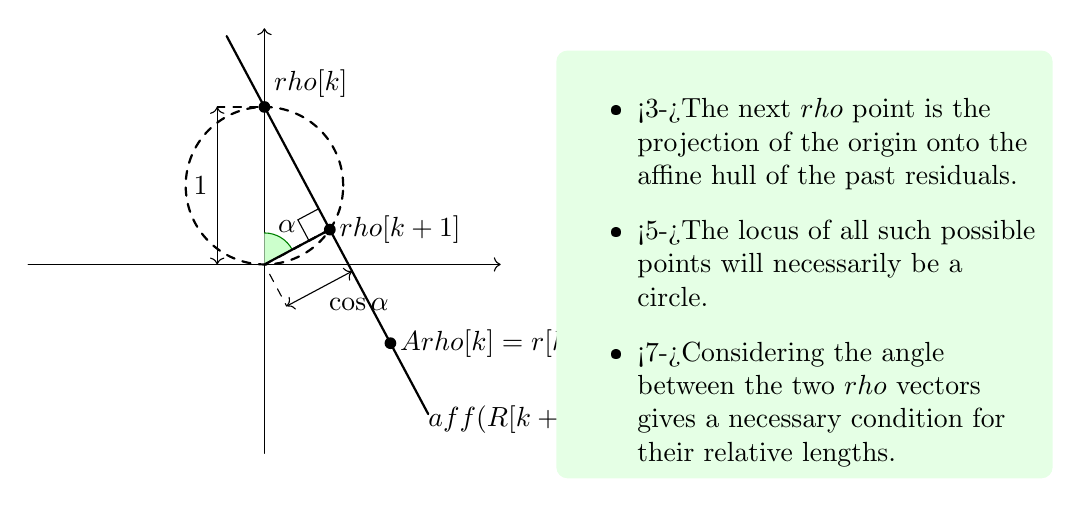
\begin{tikzpicture}[scale=2,cap=round]
  % Local definitions
  \def\costhirty{0.8660256}

  % Colors
  \colorlet{anglecolor}{green!50!black}
  \colorlet{sincolor}{red}
  \colorlet{tancolor}{orange!80!black}
  \colorlet{coscolor}{blue}

  % Styles
  \tikzstyle{axes}=[]
  \tikzstyle{important line}=[very thick]
  \tikzstyle{information text}=[rounded corners,fill=green!10,inner sep=1ex]
\tikzset{
  residual/.style={
    circle,
    fill,
    inner sep=1.5pt
  }
}

\node (origin) at (0,0) {};

  % The graphic
  \begin{scope}[style=axes]
    \draw[->] (-1.5,0) -- (1.5,0);
    \draw[->] (0,-1.2) -- (0,1.5);
  \end{scope}

  \onslide<1->{
  \node[residual] (rho_k) at (0,1) { };
  \node[above right] at (rho_k) {$\gls{rho}[k]$};}

  \onslide<2-5>{
  \node[residual] (r_k) at (0.8,-0.5) { };
  \node[right] at (r_k) {$\gls{A}\gls{rho}[k] =\gls{r}[k]$};}

  \onslide<3-5>{
  \draw[thick]
  ($(rho_k)!-0.3!(r_k)$)
  -- node[pos=0.95, below right] {$\gls{aff}(\gls{R}[k+1])$}
  ($(rho_k)!1.3!(r_k)$);}

  \onslide<4-5>{
  \coordinate (foot) at ($(rho_k)!(0,0)!(r_k)$);
  \draw[thick, dashed] (0,0) -- (foot);
  \pic[draw, angle radius=3mm] {right angle = rho_k--foot--origin};
  }

  \onslide<5->{
   \node[residual] (rho_kp1) at (foot) { };
  \node[right] at (rho_kp1) {$\gls{rho}[k+1]$};
  }

  \onslide<6>{
  \draw[thick,dashed] (0,0.5) circle (0.5cm);
  }

\onslide<7->{
  \pic[
    draw=anglecolor,
    fill=green!20,
    angle radius=4mm,
    "$\alpha$",
    angle eccentricity=1.4
  ] {angle = rho_kp1--origin--rho_k};
  \draw[thick] (0,0) -- (foot);

}

\onslide<8->{
\draw[dashed] (origin) -- ($(origin)!3mm!270:(foot)$);
\draw[dashed] (foot)   -- ($(foot)!3mm!90:(origin)$);

\draw[<->]
  ($(origin)!3mm!270:(foot)$)
  --
  node[midway,below right] {$\cos\alpha$}
  ($(foot)!3mm!90:(origin)$);

\draw[dashed] (origin) -- ($(origin)!3mm!90:(rho_k)$);
\draw[dashed] (rho_k)   -- ($(rho_k)!3mm!270:(origin)$);

\draw[<->]
  ($(origin)!3mm!90:(rho_k)$)
  --
  node[midway,left] {$1$}
  ($(rho_k)!3mm!270:(origin)$);
}

\onslide<3->{
  \draw[xshift=1.85cm] node [right,text width=6cm,style=information text]
    {\begin{itemize}\item \onslide<3->{The next $\gls{rho}$ point is the projection of the origin onto the affine hull of the past residuals.}

    \item \onslide<5->{The locus of all such possible points will necessarily be a circle.}

    \item \onslide<7->{Considering the angle between the two $\gls{rho}$ vectors gives a necessary condition for their relative lengths.}
    \end{itemize}
    };}
\end{tikzpicture}
        \caption{2D intuition}
        \label{fig:2dpicture}
    \end{figure}
\end{frame}

\begin{frame}{Behaviour of $\gls{rho}[i]$ in higher dimensions}

    % Considering the matrix, $\gls{Mmat}[k]$, i.e,
    % \begin{equation}
    %     \gls{Mmat}[k] = 
    %     \begin{bmatrix}
    %         \gls{rho}[1] & \gls{rho}[2] & \cdots & \gls{rho}[k]
    %     \end{bmatrix},
    % \end{equation}
    % now assume $\|\gls{rho}[1]\| = 1$, and denote the ratios between subsequent norms as, 
    % \begin{equation}
    %     \gls{c}[i] := \frac{\|\gls{rho}[i+1]\|}{\|\gls{rho}[i]\|},
    % \end{equation}
    % then the vector of norms can be written as,
    % \begin{equation}
    %     \gls{ctildevec}[k] := \begin{bmatrix}
    %         \|\gls{rho}[1]\| & \|\gls{rho}[2]\| & \cdots & \|\gls{rho}[k]\|
    %     \end{bmatrix}^T
    %     = 
    %     \begin{bmatrix}
    %         1 & \gls{c}[1] & \gls{c}[1]\gls{c}[2] & \cdots
    %         &\gls{c}[1]\gls{c}[2]\cdots\gls{c}[k-1]
    %     \end{bmatrix}^T
    % \end{equation}
    With some assumptions we factor out the magnitudes from the Gram matrix, i.e.,
    \begin{equation}
        \gls{Mmat}[k]^T\gls{Mmat}[k] =
        \operatorname{diag}(\gls{ctildevec}[k])\gls{KMSmat}[k]\operatorname{diag}(\gls{ctildevec}[k]),
    \end{equation}
    then the middle matrix has the following nice structure,
    \begin{equation}
        \gls{KMSmat}[k] :=
        \begin{pmatrix}
            1 & \gls{c}[1] & \gls{c}[1]\gls{c}[2] & \gls{c}[1]\gls{c}[2]\gls{c}[3] & \cdots & \prod_{j=1}^{k-1}\gls{c}[j] \\
            \gls{c}[1] & 1 & \gls{c}[2] & \gls{c}[2]\gls{c}[3] & \cdots & \prod_{j=2}^{k-1}\gls{c}[j] \\
            \gls{c}[1]\gls{c}[2] & \gls{c}[2] & 1 & \gls{c}[3] & \cdots & \prod_{j=3}^{k-1}\gls{c}[j] \\
            \gls{c}[1]\gls{c}[2]\gls{c}[3] & \gls{c}[2]\gls{c}[3] & \gls{c}[3] & 1 & \cdots & \prod_{j=4}^{k-1}\gls{c}[j] \\
            \vdots & \vdots & \vdots & \vdots & \ddots & \vdots \\
            \prod_{j=1}^{k-1}\gls{c}[j] & \prod_{j=2}^{k-1}\gls{c}[j] & \prod_{j=3}^{k-1}\gls{c}[j] & \prod_{j=4}^{k-1}\gls{c}[j] & \cdots & 1
        \end{pmatrix}.
    \end{equation}

    {\footnotesize This is something like an inhomogeneous \gls{kms} \parencite{Kac1953}, (or the
    correlation matrix of a time-varying AR(1) process \parencite{Charbonnier1987}).}

% \appxnote{More justification for this decomposition}{
%     Since we have shown the hull equivalency we need to show that the $\gls{vecalpha}$ coefficient returned when using this Gram matrix, i.e.,
%     \begin{equation}\label{eqn:vecalphai}
%         \gls{vecalpha} = \frac{(\gls{Mmat}[k]^T\gls{Mmat}[k])^{-1}\gls{e}}{\gls{e}^T(\gls{Mmat}[k]^T\gls{Mmat}[k])^{-1}\gls{e}}.
%     \end{equation}
%     is equal to $\gls{e}_k$ (the $k$th standard basis vector). This is straightforward since the explicit form for the inverse of the matrix is easily calculated (see decomposition earlier in the slides).
%     }

\end{frame}

% \begin{frame}{Facts about the $\gls{KMSmat}[k]$ matrix}
%
%     Given the matrices, 
%     \begin{equation}
%         \gls{KMSD}[k] = \operatorname{diag}(\begin{bmatrix}
%             1 & 1-\gls{c}[1]^2 & 1 - \gls{c}[2]^2&\cdots & 1-\gls{c}[k-1]^2
%         \end{bmatrix}^T),
%     \end{equation}
%     \begin{equation}
%         \gls{KMSLtilde}[k]^{-1} = \begin{pmatrix}
%             1 & 0 & 0 & \cdots & 0 & 0 \\
%             -\gls{c}[1] & 1 & 0 & \cdots  & 0 & 0 \\
%             0 & -\gls{c}[2] & 1 & \cdots & 0 & 0 \\
%             \vdots & \vdots & \vdots & \ddots & \vdots & \vdots \\
%             0 &  0 & 0 & \cdots & 1 & 0 \\
%             0 & 0 & 0 & \cdots & -\gls{c}[k-1] & 1
%         \end{pmatrix}
%     \end{equation}
%
%     we have the decomposition,
%     \begin{equation}
%         \gls{KMSmat}[k] = \gls{KMSLtilde}[k] \gls{KMSD}[k] \gls{KMSLtilde}[k]^T.
%     \end{equation}
%
% \end{frame}

\begin{frame}{Optimality theorem}

    Letting $\gls{KMSL}[k]\gls{KMSL}[k]^T = \gls{KMSmat}[k]$, (the Cholesky
    decomposition), we denote the last row of $\gls{KMSL}[k]$ as,
    \begin{equation}
        \gls{KMSl} = \gls{KMSL}[k]^T \gls{e}_k.
    \end{equation}
    Now if (after factoring out vector norms), $\gls{Mtildemat}[k]^T\gls{Mtildemat}[k]$
    has a Cholesky decomposition with last row, $\gls{KMSlpert}$, then we have

    \begin{theorem}\label{thm:perturbation}
        \begin{equation}
            \|\gls{rho}[k]\|^2 =
            \frac{1}{\gls{e}^T(\gls{Mtildemat}[k]^T\gls{Mtildemat}[k])^{-1}\gls{e}} =
            \frac{\|\gls{r}[k-1]\|^2}{\gamma},
        \end{equation}
        with,
        \begin{equation}
            \gamma := 1 +
            \left(\frac{1-\gls{KMSlpert}\cdot\gls{KMSl}}{\gls{KMSlpert}\cdot\gls{e}_k}\right)^2
            +
            2(\gls{KMSl}\cdot\gls{e}_k)\left(\frac{1-\gls{KMSlpert}\cdot\gls{KMSl}}{\gls{KMSlpert}\cdot\gls{e}_k}
            \right)\geq
            1
        \end{equation}
    \end{theorem}

\end{frame}

\begin{frame}{Implications}

    \begin{itemize}
        \item In other words if the next residual $\gls{r}[k]$ leads to a Gram matrix
            that is of a different form than our inhomogeneous \gls{kms} matrix then we
            have that $\gls{rho}[k+1]$ will be smaller than $\gls{r}[k]$ by a set
            factor.
        \item This is a similar idea to the stage-$k$ gain defined in \parencite{Evans2020}.
    \end{itemize}

% \appxnote[allowframebreaks]{Details about perturbation argument}{
%     We start with $\gls{KMSL}$, the factor in the Cholesky decomposition. We wish to find out how the inverse changes with respect to a rank-1 update given by,
%     \begin{equation}
%         \gls{KMSL} \leftarrow \gls{KMSL} + \gls{e}_k (\gls{KMSlpert} - \gls{KMSl}).
%     \end{equation}
%     Now note the following elementary facts, 
%     \begin{equation}
%         \gls{KMSl}^T \gls{KMSL}^{-1} = \gls{e}_k^T, \quad
%         \gls{KMSL}^{-1}\gls{e}_k = \frac{\gls{e}_k}{\gls{KMSl}\cdot\gls{e}_k}.
%     \end{equation}
%     So that by the Sherman-Morrison formula we have,
%     \begin{equation}
%         \gls{KMSL}^{-1} \leftarrow \gls{KMSL}^{-1} + \frac{\gls{e}_k\gls{e}_k^T-\gls{e}_k\gls{KMSlpert}^T\gls{KMSL}^{-1}}{\gls{KMSlpert}\cdot\gls{e}_k}.
%     \end{equation}
%     To complete the computation we then need,
%     \begin{equation}
%         \gls{ew}_k := \begin{bmatrix}
%             \frac{1}{\|\gls{rho}[1]\|} & \frac{1}{\|\gls{rho}[2]\|} & \cdots & \frac{1}{\|\gls{rho}[k-1]\|} & \frac{1}{\|\gls{r}[k-1]\|}
%         \end{bmatrix}^T = \gls{diag}(\mathbold{v})^{-1}\gls{e},
%     \end{equation}
%     which is such that,
%     \begin{equation}
%         \|\gls{KMSL}^{-1}\gls{ew}_k\|^2 = \gls{e}^T\gls{Mtildemat}[k]\gls{Mtildemat}[k]\gls{e},
%     \end{equation}
%     where the $\gls{KMSL}^{-1}$ is the updated version!
%     Now we again have the following facts,
%     \begin{equation}
%         \gls{KMSL}^{-1}\gls{ew}_k = \frac{\gls{KMSL}^T\gls{e}_k}{\|\gls{r}[k-1]\|} = \frac{\gls{KMSl}}{\|\gls{r}[k-1]}, \quad \gls{e}_k\gls{e}_k^T \gls{ew} = \frac{\gls{e}_k}{\|\gls{r}[k-1]\|}.
%     \end{equation}
%     Giving that,
%     \begin{equation}
%         \left(\gls{KMSL}^{-1} + \frac{\gls{e}_k\gls{e}_k^T-\gls{e}_k\gls{KMSlpert}^T\gls{KMSL}^{-1}}{\gls{KMSlpert}\cdot\gls{e}_k}\right)\gls{ew} = \frac{1}{\|\gls{r}[k-1]\|}\left(\gls{KMSl}+\frac{1-\gls{KMSlpert}\cdot\gls{KMSl}}{\gls{KMSlpert}\cdot\gls{e}_k}\gls{e}_k\right).
%     \end{equation}
%     So the norm of this vector is,
%     \begin{equation}
%         \frac{1}{\|\gls{r}[k-1]\|^2} \left(1+\left[\frac{1-\gls{KMSlpert}\cdot\gls{KMSl}}{\gls{KMSlpert}\cdot\gls{e}_k}\right]^2+2(\gls{KMSl}\cdot\gls{e}_k)\left[\frac{1-\gls{KMSlpert}\cdot\gls{KMSl}}{\gls{KMSlpert}\cdot\gls{e}_k}\right]\right).
%     \end{equation}
% }
\end{frame}

\begin{frame}{\gls{aa} no improvement examples}

    When all the $\gls{c}[i]$ are constant (say $\gls{c}$) we can find an orthogonal
    matrix $\gls{A}$ such that \gls{aa} applied to $\gls{c}\gls{A}$ with an appropriate
    intial point produces exactly the same iterates as \gls{pi}.

    \begin{itemize}
        \item Works for both restarted, and windowed \gls{aa} (with some assumptions).
        \item In essence the ``rotation'' of vectors has to match their ``shrinking''.
    \end{itemize}

    % \appxnote{Finding the no improvement examples}{
    %     When all the $\gls{c}[i]$ are constant we get exactly the \gls{kms} matrix. Can then take the Cholesky factorisation of this, and use the vectors in this to create a moment problem \cite{Vorobyev1965}. Adding the additional assumptions for orthogonality gives a well-defined linear map. 
    %
    %     Finally, in the restarted and windowed cases the orthogonality ensures that inner products remain the same no matter how much the map is applied. Thus in the asymptotic case the no-improvement idea holds.
    %     }

\end{frame}

\begin{frame}{Where to go from here?}

    \begin{itemize}
        \item We obtain a different expression for the $k$-stage gain than
            \cite{Evans2020}, we can look at when this can be bounded for some specific
            examples of linear maps.
        \item Can we provide a complete characterisation of when \gls{aa} produces no
            improvement over \gls{pi}.
        \item Comparisons to the polynomial based bounds.
        \item \cite{Feng2024a} did some work on the alternating \gls{aa}/\gls{pi}
            variant (basically \gls{aa} applied to powers of map). It will be
            interesting to see if there is a way to give an expression for the optimal
            power.
    \end{itemize}

    % \appxnote{Example of improvement by alternating}{
    %     Just in the 2D case, we compare two procedures, either:
    %     \begin{itemize}
    %         \item the process of doing windowed \gls{aa} with history parameter 1 (i.e. we keep taking Anderson steps based on only the last residual); or,
    %         \item taking two \gls{pi} steps and then doing \gls{aa} with only this point and the first point.
    %     \end{itemize}
    %
    %     Doing this for the maps $\cos(\theta) R(\theta)$, ($R(\theta)$ is a rotation by $\theta$ - the case where \gls{aa} is just \gls{pi}), with $\theta \in \left(0,\frac{\pi}{2}\right)$, gives the following improvement when doing the two \gls{pi} steps and then \gls{aa},
    %
    %     \begin{figure}
    %         \centering
    %         \begin{tikzpicture}[scale=0.4]
\begin{axis}[
    domain=0:pi/2,
    samples=500,
    smooth,
    xmin=0+0.1, xmax=pi/2,
    ymin=-0.5, ymax=1.5,
    xlabel={$ \theta $},
    ylabel={},
    axis lines=left,
    enlargelimits=false,
    clip=true,
    xtick={0,pi/8,pi/4,3*pi/8,pi/2},
    xticklabels={
        $0$,
        $\frac{\pi}{8}$,
        $\frac{\pi}{4}$,
        $\frac{3\pi}{8}$,
        $\frac{\pi}{2}$
    },
]
\addplot[
    thick,
]
{sin(deg(2*x)) / sqrt(1 + (cos(deg(x))^2)^2 - 2*(cos(deg(x))^2)*cos(deg(2*x)))};
\end{axis}
\end{tikzpicture}
    %         \caption{Ratio of the alternating iterate to the standard \gls{aa} iterate after the same number of function evaluations.}
    %         \label{fig:alternatingimprovement}
    %     \end{figure}
    %
    %     }

\end{frame}

\appendix

\begin{frame}[shrink=35]
  \frametitle{References}

  \tiny
  \printbibliography

\end{frame}

\printappxnotes

\end{document}
